\documentclass[12pt,a4paper,oneside]{report}
\usepackage[T1]{fontenc}
\usepackage{mathptmx}
\usepackage[left=30mm,right=25mm,top=25mm,bottom=25mm]{geometry}

\usepackage{titlesec}
\usepackage{fancyhdr}
\setlength{\headheight}{30pt}
\setlength{\headsep}{12pt}


\usepackage{graphicx,array,longtable,pdflscape,setspace}
% Packages added for this report's equations, diagrams, charts and algorithms.
\usepackage{amsmath,amssymb}
\usepackage{xcolor}
\usepackage{tikz}
\usetikzlibrary{positioning,arrows.meta,shapes.geometric,fit,backgrounds,calc}
\usepackage{pgfplots}
\pgfplotsset{compat=1.18}
\usepackage{algorithm}
\usepackage{algpseudocode}
\usepackage{caption}
\captionsetup[table]{skip=6pt}
\usepackage{enumitem}
\setlist{itemsep=1pt,topsep=3pt}
\usepackage{xurl}
\usepackage[hidelinks]{hyperref}
\onehalfspacing
\setlength{\parindent}{0pt}
\setlength{\parskip}{4pt}
\setcounter{tocdepth}{1}
\renewcommand{\contentsname}{Table of Contents}
\newcommand{\institutionlogo}[1]{\IfFileExists{amrita-logo.png}{
\includegraphics[width=#1]{amrita-logo.png}}{\fbox{\parbox{#1}{\centering Amrita Vishwa Vidyapeetham\\Place amrita-logo.png beside this file}}}}
\newcommand{\ProjectTitle}{Adaptive Multi-Agent AI Tutoring System for Personalized Programming Education}
\fancypagestyle{project}{%
  \fancyhf{}
  \fancyhead[C]{\parbox{\textwidth}{\centering\small\nouppercase{\ProjectTitle}}}
  \fancyfoot[C]{\thepage}
  \renewcommand{\headrulewidth}{0.4pt}
}
% Preliminary pages show only a page number.
\fancypagestyle{plain}{%
  \fancyhf{}
  \fancyfoot[C]{\thepage}
  \renewcommand{\headrulewidth}{0pt}
}
\newcommand{\EnableProjectHeaders}{%
  \pagestyle{project}%
  % report uses plain style on chapter-opening pages.
  \fancypagestyle{plain}{%
    \fancyhf{}
    \fancyhead[C]{\parbox{\textwidth}{\centering\small\nouppercase{\ProjectTitle}}}
    \fancyfoot[C]{\thepage}
    \renewcommand{\headrulewidth}{0.4pt}
  }%
}
\titlespacing*{\chapter}{0pt}{0pt}{16pt}
\titlespacing*{\section}{0pt}{10pt}{4pt}
\titlespacing*{\subsection}{0pt}{8pt}{3pt}
\titlespacing*{\subsubsection}{0pt}{6pt}{3pt}
\raggedbottom
\setlength{\emergencystretch}{3em}

% Report-wide helpers.
\newcolumntype{R}[1]{>{\raggedright\arraybackslash}p{#1}}
% Monospace names may break after an underscore or a slash, so long identifiers fit in table cells.
\newcommand{\code}[1]{\begingroup\ttfamily\renewcommand{\_}{\textunderscore\allowbreak}#1\endgroup}
\tikzset{
  box/.style={draw, rounded corners=2pt, align=center, font=\small, inner sep=4pt, fill=white},
  agent/.style={box, fill=blue!6, minimum width=3.1cm, minimum height=0.9cm},
  store/.style={draw, cylinder, shape border rotate=90, aspect=0.18, align=center, font=\small, fill=gray!10, minimum width=2.4cm, minimum height=1.1cm},
  arrow/.style={-{Stealth[length=2.2mm]}, thick},
  darrow/.style={{Stealth[length=2.2mm]}-{Stealth[length=2.2mm]}, thick},
  note/.style={font=\footnotesize, align=center, text=black!70},
}
\newcommand{\screenshot}[3]{%
  \begin{figure}[htbp]\centering
  \includegraphics[width=\textwidth]{figures/screens/#1}
  \caption{#2}\label{#3}
  \end{figure}}

\begin{document}
\pagestyle{empty}

{\centering \Large\bfseries \ProjectTitle{}\par}
{\centering Project report submitted in partial fulfilment of the requirements for the award of the degree of\par}
{\centering \textbf{BACHELOR OF TECHNOLOGY}\par}
{\centering in\par}
{\centering \textbf{COMPUTER SCIENCE AND ENGINEERING}\par}
{\centering Submitted by\par}
{\centering \fontsize{14}{18}\selectfont
Kataru Reddy Eswar \quad AM.SC.U4CSE23126\par}

{\centering \fontsize{14}{18}\selectfont
Bharath Bommineni \quad AM.SC.U4CSE23112\par}

{\centering \fontsize{14}{18}\selectfont
Chimmili Lokesh \quad AM.SC.U4CSE23114\par}

{\centering \fontsize{14}{18}\selectfont
Ramisetti Gowtham Tej \quad AM.SC.U4CSE23144\par}

{\centering \fontsize{14}{18}\selectfont
Under the guidance of\par
Ms. Anju Sukumar\par
[Guide designation]\par}

{\centering \institutionlogo{4.5in}\par}

{\centering \textbf{AMRITA SCHOOL OF COMPUTING}\par}
{\centering \textbf{AMRITA VISHWA VIDYAPEETHAM}\par}
{\centering \textbf{AMRITAPURI CAMPUS}\par}
{\centering \textbf{KOLLAM 690525}\par}
{\centering \textbf{NOVEMBER 2026}\par}


\clearpage
{\centering \institutionlogo{3.7in}\par}
{\centering \textbf{DEPARTMENT OF COMPUTER SCIENCE AND ENGINEERING}\par}
{\centering Amrita School of Computing, Amritapuri Campus\par}
{\centering \Large\bfseries BONAFIDE CERTIFICATE\par}
This is to certify that the project report entitled ``\ProjectTitle{}'', submitted by Kataru Reddy Eswar (AM.SC.U4CSE23126), Bharath Bommineni (AM.SC.U4CSE23112), Chimmili Lokesh (AM.SC.U4CSE23114) and Ramisetti Gowtham Tej (AM.SC.U4CSE23144), in partial fulfilment of the requirements for the award of the degree of Bachelor of Technology in Computer Science and Engineering at Amrita Vishwa Vidyapeetham, is a bonafide record of the work carried out by them under my guidance and supervision at Amrita School of Computing, Amritapuri, during Semester 7 of the academic year 2026 - 2027.

\begin{tabular}{p{.46\textwidth}p{.46\textwidth}} Ms. Anju Sukumar & [Coordinator name] \\ Project Guide & Project Coordinator \\ Signature \hrulefill & Signature \hrulefill \\[20pt] [Chairperson name] &  \\ Chairperson, CSE & Reviewers \\ Signature \hrulefill & Signature \hrulefill \end{tabular}
\\
\\
\\ Place: Amritapuri\\
Date: [DD Month YYYY]
\clearpage
\thispagestyle{empty}

{\centering
\institutionlogo{3.7in}\par
\vspace{0.4cm}
\textbf{DEPARTMENT OF COMPUTER SCIENCE AND ENGINEERING}\par
Amrita School of Computing, Amritapuri Campus\par
\vspace{0.6cm}
{\Large\bfseries DECLARATION\par}
}

\vspace{0.5cm}

\noindent
{\sloppy
We, Kataru Reddy Eswar (AM.SC.U4CSE23126),
Bharath Bommineni (AM.SC.U4CSE23112),
Chimmili Lokesh (AM.SC.U4CSE23114) and
Ramisetti Gowtham Tej (AM.SC.U4CSE23144),
hereby declare that the project entitled
``\ProjectTitle{}'' is a record of our original work
carried out under the guidance of Ms. Anju Sukumar, [Guide designation],
Department of Computer Science and Engineering,
Amrita Vishwa Vidyapeetham, Amritapuri.
To the best of our knowledge, this work has not formed the
basis for the award of any degree, diploma, fellowship or
similar qualification to any candidate at any university.
All sources and contributions of others have been
appropriately acknowledged.\par}

\vspace{0.5cm}

\noindent
Place: Amritapuri\\
Date: [DD Month YYYY]

\vspace{0.7cm}

\noindent
\begin{tabular}{@{}p{0.60\textwidth}p{0.34\textwidth}@{}}
\textbf{Student details} & \textbf{Signature of the student} \\[14pt]

Kataru Reddy Eswar\newline
AM.SC.U4CSE23126
& \rule{0.30\textwidth}{0.4pt} \\[18pt]

Bharath Bommineni\newline
AM.SC.U4CSE23112
& \rule{0.30\textwidth}{0.4pt} \\[18pt]

Chimmili Lokesh\newline
AM.SC.U4CSE23114
& \rule{0.30\textwidth}{0.4pt} \\[18pt]

Ramisetti Gowtham Tej\newline
AM.SC.U4CSE23144
& \rule{0.30\textwidth}{0.4pt}
\end{tabular}

\vspace{0.8cm}

\noindent
\textbf{Project Guide:} Ms. Anju Sukumar

\vspace{0.5cm}

\noindent
\textbf{Signature of the Project Guide:}
\rule{4cm}{0.4pt}

\clearpage

\clearpage
% Arabic numbering continues through the preliminary pages and chapters.
\clearpage
\pagenumbering{roman}
\pagestyle{plain}

\phantomsection
\addcontentsline{toc}{chapter}{Acknowledgement}
{\centering \Large\bfseries ACKNOWLEDGEMENT\par}
We are sincerely grateful to our project guide, Ms. Anju Sukumar, Department of Computer Science and Engineering, for guiding us throughout this project. She kept asking us how a tutor should decide when to help a beginner and how much, and those questions shaped the design of the scaffolding and reflection components. She also reviewed our progress at each stage, and that kept our attention on the learner as much as on the technology.

We thank the Project Coordinator and the Chairperson of the Department of Computer Science and Engineering for organising the project reviews and for their feedback. We also thank the faculty members of the department. This work builds on their courses in programming, databases, software engineering and artificial intelligence.

We are grateful to Amrita School of Computing, Amrita Vishwa Vidyapeetham, Amritapuri Campus, for the academic environment and the facilities we used for this project.

We acknowledge the authors and maintainers of the open-source software used in this project, including Python, FastAPI, LangGraph, PostgreSQL, ChromaDB, React and Docker, and the researchers whose published work we review and cite in this report.

Finally, we thank our families and friends for their encouragement and their patience while we worked on this.

\vspace{1cm}
\begin{flushright}
Kataru Reddy Eswar\\
Bharath Bommineni\\
Chimmili Lokesh\\
Ramisetti Gowtham Tej
\end{flushright}


\clearpage
\phantomsection
\addcontentsline{toc}{chapter}{Abstract}
{\centering \Large\bfseries ABSTRACT\par}
A large language model (LLM) assistant will write out the full answer to a beginner's programming exercise in a few seconds. A learner who copies that answer has finished the exercise but skipped the reasoning it was set to practise, and most LLM tutors also keep no lasting record of what the learner knows. In this project we designed and built CodePath, a web-based tutor for novice Python programmers. It implements the Cognitive-State Guided Multi-Agent Adaptive Scaffolding Framework (CSMASF). Six agents run in a cyclic LangGraph workflow after every run, submission or help request. The Diagnostic agent analyses the test results and the program's syntax tree. The Cognitive State agent estimates topic mastery with Bayesian Knowledge Tracing and also tracks confusion, workload and progress. Past situations like the current one are found by the Similar Learner Retrieval agent, which searches ChromaDB by cosine similarity. The Adaptive Scaffolding agent applies the Dynamic Scaffolding Decision Algorithm (DSDA) to decide whether to help, at which of five levels and with which strategy, and then generates the hint and validates it. A Reflection agent asks the learner about their own code and replies to the answer, and a Learning Planner orders practice by technique and difficulty. A hint never contains a complete solution and is never repeated, and the amount of help grows only when the learner asks. The system has 496 verified problems across 17 topics, with 15,717 tests. On the final code, 551 backend tests, 59 browser tests and 21 frontend unit tests passed. We also ran an audit that drives nine real scenarios through all the agents, and it passed all 37 of its behavioural checks. We have not yet carried out a study with real learners, so the effect on learning is still to be measured. The project contributes to United Nations Sustainable Development Goal 4, Quality Education, through Target 4.4: it helps novices acquire programming skills relevant to employment while they stay responsible for their own reasoning.

\vspace{0.3cm}
\textbf{Keywords:} Intelligent tutoring systems; Multi-agent systems; Adaptive scaffolding; Knowledge tracing; Programming education; Large language models



\clearpage
\tableofcontents
\clearpage
\phantomsection
\addcontentsline{toc}{chapter}{List of Figures}
\listoffigures
\clearpage
\phantomsection
\addcontentsline{toc}{chapter}{List of Tables}
\listoftables
\clearpage
\pagenumbering{arabic}
\pagestyle{plain}
\EnableProjectHeaders
\chapter{Introduction}
\section{Background and motivation}
Most engineering and science students now have to learn programming, and many of them find the first course hard. When a beginner gets stuck, the help that works is help that comes quickly and fits what they already understand. A human tutor can give this, but one tutor cannot cover a large class. Intelligent tutoring systems (ITS) were developed to make up for that. In a widely cited review, VanLehn found that step-based tutoring systems raised learning outcomes by an effect size of 0.76 against no tutoring, which is close to the 0.79 of human tutoring \cite{vanlehn2011}.

The \emph{amount} of help matters as well as its correctness, and two ideas from learning science explain why. The first is \emph{scaffolding}, described by Wood, Bruner and Ross. The tutor controls the parts of a task that are beyond the learner so that the learner can complete the rest, and withdraws that support as the learner becomes more competent \cite{wood1976}. The second is Sweller's cognitive load theory. Problem solving already places heavy demands on working memory, so a hint that is too long, or hints that arrive too often, can get in the way of learning \cite{sweller1988}. Research on help seeking in tutoring systems adds a caution. Learners do not always use on-demand help well, and teaching them to seek help more deliberately does not automatically improve their learning \cite{aleven2016}.

Large language model (LLM) assistants have made the question more pressing. They answer almost any programming question at once, they give everyone the same kind of help, and they readily produce complete solutions. An eleven-week classroom study of PyTutor, a ChatGPT-based tutor, found clear benefits for students with weak foundations. The same study found a risk of over-reliance that may hinder independent problem solving \cite{yang2024}. Tools such as CodeHelp and CodeAid add guardrails so that the assistant does not give away solutions \cite{liffiton2023,kazemitabaar2024}. Their published descriptions, though, do not include a lasting model of each learner that decides how much help to give.

That is the gap we worked on. We built CodePath, a tutor for novice Python programmers, on the Cognitive-State Guided Multi-Agent Adaptive Scaffolding Framework (CSMASF) proposed in our initial project submission. It has six cooperating agents. One diagnoses each attempt and one estimates the learner's state. A third looks at what helped in similar situations, and a fourth decides how much help fits. The last two prompt reflection and plan the next problem. Throughout, we wanted the tutor to behave like a patient teacher sitting beside the student, who gives only the help the student needs at that moment, never gives the full answer, and leaves the thinking to the student.

\textbf{Relevant Sustainable Development Goal.} The project is aligned with United Nations SDG 4, Quality Education: ``Ensure inclusive and equitable quality education and promote lifelong learning opportunities for all'' \cite{un2015}. The most relevant target is Target 4.4: ``By 2030, substantially increase the number of youth and adults who have relevant skills, including technical and vocational skills, for employment, decent jobs and entrepreneurship.''

The project maps to this target in four ways. The problem is that programming skill is in demand, but beginners who receive complete answers from AI tools may not develop it. Our objectives answer this directly, since the tutor adapts the amount of help to each learner and protects the learner's own reasoning (Section~\ref{sec:objectives}). The contribution is a working, open, web-based tutor with a verified 496-problem Python curriculum. It can be offered alongside a course at low cost and without a paid model, because every agent has a built-in deterministic mode. The intended beneficiaries are novice programmers, including learners who have no access to a personal tutor, and teachers, who get a class dashboard showing who may need support.

The contribution to Target 4.4 is an \emph{expected} benefit. We have built the system and verified it as software, but we have not yet measured its effect on learners' skills (Chapter~\ref{ch:results}).

\section{Objectives}\label{sec:objectives}
The five objectives come from the initial project submission. For each one, Table~\ref{tab:objectives} gives the way it is evaluated in this report, its deliverable and its status at the time of writing.

\begingroup\small
\setlength{\tabcolsep}{4pt}\renewcommand{\arraystretch}{1.2}
\begin{longtable}{|R{0.5cm}|R{3.5cm}|R{4.2cm}|R{3.0cm}|R{2.4cm}|}
\caption{Objectives, evaluation methods, deliverables and status}\label{tab:objectives}\\\hline
\textbf{No.} & \textbf{Objective} & \textbf{Evaluation method} & \textbf{Deliverable} & \textbf{Status}\\\hline\endfirsthead
\hline\textbf{No.} & \textbf{Objective} & \textbf{Evaluation method} & \textbf{Deliverable} & \textbf{Status}\\\hline\endhead
O1 & Build an adaptive tutor as several collaborating agents rather than one conversational model. & Pipeline tests confirm that all six agents run in order and receive each other's outputs; per-stage traces are inspected. & Six agents in a LangGraph workflow inside a web platform. & Achieved.\\\hline
O2 & Continuously estimate mastery, confidence, confusion, cognitive load and progress from behaviour. & Unit and pipeline tests; audit checks that unknown values stay unknown and that estimates react to repeated requests and progress. & Cognitive State agent (method \code{cs-1.2}). & Achieved as behavioural estimates; not validated against an external measure.\\\hline
O3 & Retrieve similar learners with vector cosine similarity over multidimensional profiles. & Tests of filtering, exclusion of approaches already shown, reliability thresholds and absence of identities in the output. & Retrieval agent over ChromaDB and PostgreSQL (vectors \code{sv-1}). & Achieved technically; real learner outcomes are not yet available.\\\hline
O4 & Design a scoring algorithm that selects the scaffolding level from mastery, confidence, hint history and response time. & Policy tests, including a documented worked example recomputed by the code; audit checks of escalation and timing. & DSDA, policy version \code{dsda-2.2}. & Achieved; weights are starting values, not tuned on learners.\\\hline
O5 & Test the framework's effectiveness on programming datasets. & Offline verification of every curriculum problem in the sandbox; scenario audit of all agents; planned learner study. & Verified curriculum, audit tool and evaluation plan. & Partly achieved: software behaviour verified; learning effectiveness not yet measured.\\\hline
\end{longtable}
\endgroup

Two more objectives follow from the way we wanted the tutor to behave, and they are evaluated in the same way: (i) the tutor never reveals a complete solution, reference solutions or hidden tests, and (ii) help is not repeated and does not increase unless the learner asks for it.

\section{Scope and constraints}
CodePath is meant for novice and early intermediate learners of Python, typically first-year undergraduates, and for the teachers of such courses.

The system includes the following functions.
\begin{itemize}
\item A browser workspace with an editor, separate Run, Submit and Hint actions, test results, and saved drafts.
\item A curriculum of 17 topics with lessons, 74 techniques and 496 problems.
\item The six tutoring agents, typed questions about selected lines, reflection questions and replies, and a learning plan with a route ahead.
\item Learner progress and profile pages, and a teacher dashboard.
\item Adding a question by pasting it or from a link, with suggested tests that are always labelled as suggestions.
\end{itemize}

The following are outside the scope of this phase.
\begin{itemize}
\item Languages other than Python are not offered.
\item No model is trained. Every agent is rule-based, and an LLM is optional and used only for wording.
\item No study with real learners has been carried out.
\item The large IBM Project CodeNet archive was not imported. Only its importer exists.
\end{itemize}

We assume that learners use a modern desktop or mobile browser and that the server host can run Docker containers for code execution.

We worked under three constraints.
\begin{itemize}
\item Development and testing used one laptop with 8~GB of memory, so the test suites had to be run one at a time.
\item The code-execution sandbox was tested on Docker Desktop for macOS and has not been independently audited.
\item The only model key we had carried no credit, so the LLM path was tested with a scripted stand-in.
\end{itemize}

\section{Project report organization}
Chapter~2 defines the problem and describes the limitations of existing systems. Chapter~3 reviews thirteen research works and compares them. Chapter~4 lists the functional and non-functional requirements along with the hardware, software and data used. Chapter~5 presents the architecture and then explains each agent: its inputs, its outputs and its algorithm. Chapter~6 covers the evaluation setup and criteria, the results, a comparison with existing approaches and the limitations. Chapter~7 concludes and outlines future work. The appendix gives the steps to set up and reproduce the system.

\clearpage
\chapter{Problem Definition}
\section{Problem statement}
A beginner working on a programming exercise writes some code, runs it, sees it fail and tries again, usually many times. At each of these moments a good tutor has several things to decide: what exactly went wrong in this version of the code, how much the learner already understands, whether to step in at all, and how much help to give if so. With too little help the learner stays stuck and gets frustrated. With too much help, or with the answer itself, the learner no longer has to do the thinking the exercise was set for.

The problem we address in this project is to build a tutor that makes these decisions automatically, consistently and transparently for every learner action, and that never hands over a complete solution.

For each learner action the system receives three inputs:
\begin{itemize}
\item the action itself, which is one of Run (try the code on visible examples), Submit (graded against all tests), Ask for a hint (optionally ``just a small nudge'' or ``I need more help''), or a typed question about selected lines;
\item the exact version of the learner's code and the problem it belongs to;
\item the stored history of this learner on this problem and topic, that is, earlier attempts and their results, hints already shown and whether they were followed by progress, reflection answers, and time spent.
\end{itemize}

From these it is expected to produce:
\begin{itemize}
\item a diagnosis of the attempt, with the evidence that supports it;
\item an updated estimate of the learner's state, which keeps uncertainty and says ``unknown'' where evidence is missing;
\item a help decision (wait, offer help, or show help) at a stated level, with a stated strategy and reason;
\item when help is shown, a hint that is specific to the learner's own code, different from earlier hints and free of solution code;
\item when useful, one reflection question about the learner's own reasoning, and a reply to the answer;
\item a recommendation of what to do next, with the route ahead.
\end{itemize}

There are three stakeholders. Learners need help that keeps them thinking. Teachers need to know which learners may need a conversation, without reading every submission. The institution needs a tool that is safe to run on its servers and that protects learners' data.

If the problem is left unsolved, learners who rely on instant complete answers may pass exercises and still be unable to solve similar problems alone. The PyTutor study explicitly reported this risk of over-reliance \cite{yang2024}. Teachers in large courses cannot give every learner timely individual help \cite{liffiton2023}. There is also a security side: running untrusted student code without isolation would expose the server.

\section{Existing system and limitations}
Four kinds of existing solutions are relevant here. Their limitations, as reported in the literature we reviewed, define the gap this project addresses.

The first kind is the general-purpose LLM assistant, a conversational question-and-answer tool. Such assistants are always available and fluent. However, they keep no model of the individual learner, apply the same help to everyone, and readily produce complete code.

The second kind is the LLM programming assistant with guardrails. CodeHelp \cite{liffiton2023}, CodeAid \cite{kazemitabaar2024} and RAGMan \cite{ma2024} restrict the assistant so that it explains, gives pseudo-code or answers within a course scope, and does not write solutions. All three were deployed in real courses and received positive student feedback. Their published descriptions, however, do not include a persistent learner model that decides \emph{how much} help each learner should receive, and RAGMan's retrieval draws on course material and not on what helped similar learners. PyTutor does provide a structured ladder of hints, but one of its hint types is a coding solution, and its authors observed over-reliance \cite{yang2024}.

Classical intelligent tutoring systems form the third kind. Systems such as the ACT Programming Tutor model the learner explicitly. Knowledge tracing estimates the probability that each skill has been learned, and that estimate drives mastery learning \cite{corbett1995}. Conversational tutors such as DeepTutor showed that tutoring dialogue can be delivered over the web at scale \cite{rus2015}. These systems depend on carefully authored domain models, which are expensive to build for each new subject.

The fourth kind is learner-modelling research. Deep Knowledge Tracing predicts whether a learner will answer the next exercise correctly, and does so more accurately than earlier models \cite{piech2015}. Newer work simulates learners or verifies tutoring dialogue \cite{zhan2025,wang2025}. These are methods for prediction, simulation or evaluation. Used alone, they do not decide when and how much to help a real learner in a live programming session.

Among the works we reviewed, no single system combines all of the following for live programming practice: (i) a continuously updated, explainable learner state, (ii) an explicit decision about whether and how much to help that escalates only on request and never reveals a solution, (iii) retrieval of what helped in similar learners' situations, and (iv) reflection and next-step planning that react to the learner's own answers. A survey of LLM applications in programming education reaches a related conclusion: interventions work best with scaffolding and human oversight, and fully automated approaches often miss pedagogical nuance \cite{pitts2025}. We designed CSMASF to fill this gap within an open, testable system.

\clearpage
\chapter{Literature Review}
\section{Review scope and selection}
We reviewed research in four areas: learner modelling, tutoring and hint provision for programming, LLM-based programming assistants, and multi-agent or conversational tutors. We searched the ACM Digital Library, the ACL Anthology, arXiv, the AAAI and IJCAI proceedings, and the Springer and Elsevier journal platforms. The search used combinations of the keywords \emph{intelligent tutoring system}, \emph{knowledge tracing}, \emph{programming education}, \emph{hint generation}, \emph{LLM programming assistant}, \emph{help seeking}, \emph{scaffolding} and \emph{multi-agent tutoring}.

A work was selected if it met three conditions. It had to be a primary research article in a peer-reviewed venue or a widely used preprint. It had to address learner modelling, help provision, programming practice or LLM-based tutoring. It also had to inform a specific design decision in CSMASF. The publication period is 1995 to 2025. We reviewed thirteen works. Nine were listed in the initial project submission, and we added four to cover the foundations of knowledge tracing \cite{corbett1995}, help-seeking research \cite{aleven2016}, guardrails for LLM help \cite{liffiton2023} and multi-agent LLM tutoring \cite{schmucker2024}.

We checked the bibliographic details of each work against its publisher or index record (DOI, ACL Anthology, IJCAI, arXiv, Crossref or OpenAlex). Findings are reported as stated in each work's abstract or published record. Numerical values are given only where they appear there or, for Deep Knowledge Tracing, in its results table. Where a detail is not stated in the material we consulted, we say so and do not assume it.

\section{Descriptive review of literature works}
The works are presented in order of publication year.

\clearpage
\subsection{Knowledge tracing}
Corbett and Anderson's ``Knowledge tracing: Modeling the acquisition of procedural knowledge'' (1995) \cite{corbett1995} asks how a tutor can model a student's knowledge state as it changes during skill acquisition. The setting is the ACT Programming Tutor, with which students learn to write short programs. The tutor has a cognitive model of programming made of production rules (the ``ideal student model'', grounded in ACT-R theory). In \emph{knowledge tracing}, while the student works, the tutor maintains for every rule an estimate of the probability that the student has learned it. Each rule is assumed to be in one of two states, learned or not learned, and the model has parameters for initial knowledge, the chance of learning at each opportunity, guessing and slipping. The estimates drive mastery learning, in which the tutor presents an individualised sequence of exercises until each rule is mastered. To assess knowledge tracing, the authors used its estimates to predict students' performance on test exercises, and they report that the model predicts that performance well. The approach needs a hand-authored rule model for each domain, and that is costly to build. We took the mastery model of our Cognitive State agent directly from this paper. The agent uses the same two-state update with fixed guess, slip and learning parameters, because it is interpretable and needs no training data.

\subsection{Deep knowledge tracing}
``Deep Knowledge Tracing'' by Piech et al. (2015) \cite{piech2015} takes up the same task, modelling a student's knowledge as they work through exercises, for large online learning platforms. The authors use recurrent neural networks, specifically long short-term memory (LSTM) networks. These learn from response sequences and need no expert annotation of the skills each exercise requires. The study uses simulated students, Khan Academy mathematics data (47,495 students, 69 exercise tags, about 1.4 million answers) and the ASSISTments benchmark (15,931 students, 124 exercise tags, about 526 thousand answers). The model is evaluated on predicting the next response, measured by the area under the ROC curve (AUC) with five-fold cross-validation on the real datasets. On the Khan data the reported AUC is 0.85, against 0.68 for standard Bayesian Knowledge Tracing (BKT). On ASSISTments it is 0.86 against the best previously reported 0.69, a 25\% gain, and on simulated data the model reached 0.82 against 0.54 for BKT. For tutoring, the main limitation is that the model predicts performance but does not itself decide what help to give. Its internal state is also less directly interpretable than BKT's parameters. BKT, which is the baseline in this paper, is the model we kept, because it is interpretable. A learned model becomes an option for us once real interaction data exists.

\clearpage
\subsection{DeepTutor}
Rus, Niraula and Banjade (2015) describe their system in ``DeepTutor: An Effective, Online Intelligent Tutoring System That Promotes Deep Learning'' \cite{rus2015}. Their question is how educational technology can deliver instruction tailored to each learner. DeepTutor is a conversational intelligent tutoring system delivered as a web application, so learners can use it at any time from a browser-connected device. It was used in large-scale experiments with high-school students, and the authors report these experiments as evidence that conversational intelligent tutoring can work at scale over the web. The published abstract does not give detailed metrics. For our purposes the system has two limitations: it predates current LLMs, and it is not designed for programming practice with code execution. What we took from it is that dialogue-based tutoring can be delivered at scale through the web. This supports CodePath's browser-based design and its conversational reflection step.

\subsection{Help seeking with intelligent tutors}
In ``Help Helps, But Only So Much: Research on Help Seeking with Intelligent Tutoring Systems'' \cite{aleven2016}, Aleven, Roll, McLaren and Koedinger (2016) study how learners seek and use on-demand help in intelligent tutoring systems. They built the Help Tutor, an agent that gave students real-time, in-context feedback on their help-seeking behaviour. Behind it is a knowledge-engineered, rule-based executable model of help seeking. The Help Tutor was evaluated in a classroom study of students' help-seeking behaviour and domain learning outcomes, and the paper adds a theoretical analysis and a review of later empirical work. The feedback did make students use on-demand help more deliberately, and this effect persisted after the feedback stopped. It did not improve domain-level learning. The authors now place less weight on on-demand, principle-based help during problem solving, although they still recommend that tutors include it. They describe helping students become better self-regulated learners as an open challenge. Three decisions in our project come from this paper. Help that the learner did not request is offered and is shown only if the learner accepts it. Help climbs only when the learner asks. And the help itself is designed to keep the learner thinking.

\clearpage
\subsection{Project CodeNet}
Puri et al. (2021) present ``Project CodeNet: A Large-Scale AI for Code Dataset for Learning a Diversity of Coding Tasks'' \cite{puri2021} in response to the lack of large, diverse datasets for training AI models on coding tasks. CodeNet is a dataset of over 14 million code samples, about 500 million lines of code, in 55 programming languages. The samples are submissions to online programming problems. They are annotated to support code similarity and classification, translation between languages, and runtime and memory improvement, and sample input and output tests are provided for 98.5\% of them. The authors supply preprocessing tools that turn source code into model inputs. They evaluate the dataset by reporting baseline results for code classification and code similarity. CodeNet contains submissions and their outcomes but no records of tutoring, hints or learner states, so by itself it does not support learner modelling or tutoring. For us it is a candidate data source for offline evaluation. CodePath includes a CodeNet importer that aggregates problem statistics, and we tested it on a fixture, but the archive itself was not imported in this phase.

\subsection{CodeHelp}
``CodeHelp: Using Large Language Models with Guardrails for Scalable Support in Programming Classes'' by Liffiton, Sheese, Savelka and Denny (2023) \cite{liffiton2023} is about large computing classes, where students need timely help but should not be encouraged to over-rely on LLMs. CodeHelp is an LLM-based tool with guardrails, so it helps students without revealing solutions. It has instructor-facing features and uses a sequence of prompting strategies to keep its outputs suitable for students. The tool was used in a first-year computer and data science course with 52 students, and their interactions were collected over 12 weeks. The evaluation covers usage patterns and student perceptions and includes the instructor's reflections. Students valued the tool's availability and its help in resolving errors. For instructors it was easy to deploy, and it complemented their support without replacing it. The published description does not include a per-learner model that adapts the amount of help over time. CodePath's rule that help never contains a solution comes from this work, and so does its validator, which checks every hint before it is shown.

\clearpage
\subsection{CodeAid}
Kazemitabaar et al. (2024) report on a classroom deployment in ``CodeAid: Evaluating a Classroom Deployment of an LLM-based Programming Assistant that Balances Student and Educator Needs'' \cite{kazemitabaar2024}. They wanted an LLM assistant that gives students helpful, technically correct support without revealing code solutions. CodeAid answers conceptual questions, produces pseudo-code with explanations and suggests fixes for incorrect student code. It was deployed for 12 weeks in a course with 700 students. The authors analysed about 8,000 uses together with weekly surveys and 22 student interviews, and then interviewed eight educators. From this they derive four design considerations: exploit what AI uniquely offers, simplify query formulation while promoting cognitive engagement, avoid direct answers while encouraging motivated learning, and keep the assistant transparent and controllable for students. The published description does not include a continuous learner model or retrieval of what helped similar learners. Two CodePath features follow from this work. The typed-question feature answers from what the selected lines actually did, and the ``Why this hint?'' explanation is there for transparency.

\subsection{PyTutor}
Yang, Lin, Lin and Ogata (2024) test whether a ChatGPT-based tutoring system can help beginners learn Python, in ``Enhancing Python Learning with PyTutor: Efficacy of a ChatGPT-Based Intelligent Tutoring System in Programming Education'' \cite{yang2024}. PyTutor gives continuous guidance, problem-solving hints and code explanations. Each question has a structured set of hints covering pseudocode, cloze, basic and advanced coding solutions. In an eleven-week experiment 35 students used PyTutor and 36 did not, and the authors compared engagement, completion and success rates in in-class and after-class exercises. PyTutor was especially effective for students with weak foundations, who showed higher engagement, completion and success. The authors also identify a risk of over-reliance that may hinder independent problem-solving skills, and they recommend balanced use. A single LLM generates the help, and the hint set includes coding solutions. We took two things from this study. It supports a graded ladder of help. Its over-reliance finding is also the reason for two CodePath rules: no level contains a solution, and unrequested help is only offered.

\clearpage
\subsection{Integrating AI tutors in a programming course}
``Integrating AI Tutors in a Programming Course'' by Ma, Krone Martins and Lopes (2024) \cite{ma2024} deals with course-specific AI tutoring for programming homework. Their system, RAGMan, is LLM-powered and supports course-specific and homework-specific tutors through retrieval-augmented generation and strict instructions. It was offered in an introductory programming course with 455 students, as five homework-specific tutors that students could use if they wished. The authors evaluate usage, answer accuracy within the intended scope and student perceptions. About half of the students used the tutors, mostly for legitimate homework questions. Within scope the tutors answered accurately 98\% of the time. Of the students who used them, 78\% said the tutors helped their learning, and students valued the non-judgmental environment. The retrieval draws on course material, and the outcomes are largely self-reported. Our retrieval design differs on the first point. RAGMan retrieves course content, whereas CodePath retrieves what helped in similar \emph{learner situations}.

\subsection{Ruffle\&Riley}
Schmucker, Xia, Azaria and Mitchell (2024) look at how LLMs can lower the cost of authoring conversational tutoring systems, in ``Ruffle\&Riley: Insights from Designing and Evaluating a Large Language Model-Based Conversational Tutoring System'' \cite{schmucker2024}. Their system automatically generates an editable tutoring script from a lesson text. It then runs a learning-by-teaching format in which two LLM agents play a student and a professor. The evaluation used biology lessons in two between-subject online studies with 200 participants in total, and compared the system with simpler question-answering chatbots and a reading activity. Users found the system engaging and helpful and felt they understood the material, and they spent more time on the activity. Their short-term learning gains, however, did not differ significantly from those of the reading activity. The domain is not programming. The paper matters to us for two reasons. It shows that several cooperating agents can structure a tutoring interaction. It also cautions that engagement and perceived helpfulness are not evidence of learning, which is why this report does not claim learning gains without a learner study.

\clearpage
\subsection{CoderAgent}
Zhan et al. (2025), in ``CoderAgent: Simulating Student Behavior for Personalized Programming Learning with Large Language Models'' \cite{zhan2025}, start from a practical difficulty. Real programming data is scarce, and offline evaluation of personalised programming tutoring often does not match real learning. They propose CoderAgent, an LLM-based agent inspired by the ACT-R cognitive architecture, which simulates students' iterative programming processes. It models both programming knowledge and coding ability, and its Programming Tree of Thought breaks each step into why, how, where and what. The study uses real-world datasets, including a Python subset of CodeNet and a college-level Java dataset (CSEDM). The simulation is evaluated on four predictions: a student's next modification intention, its location, the next submission and whether that submission will be accepted. The measures are accuracy, CodeBLEU and AUC. The authors report that CoderAgent gives interpretable insights into learning trajectories and simulates students accurately. It simulates learners and does not tutor them in real time. We see it as a possible way to test tutoring policies offline before a learner study.

\subsection{TRAVER}
Wang, Dai, Zhang, Ma, Li and Chai (2025) study how LLM tutoring agents can proactively guide learners to complete predefined coding tasks, in ``Training Turn-by-Turn Verifiers for Dialogue Tutoring Agents: The Curious Case of LLMs as Your Coding Tutors'' \cite{wang2025}. Their method, Trace-and-Verify (TRAVER), has two parts. Knowledge tracing estimates the student's knowledge state, and turn-by-turn verification keeps the tutor's guidance on track. The paper also introduces DICT, an automatic evaluation protocol based on controlled student simulation and code-generation tests. The authors report that coding tutoring is challenging and that TRAVER achieves a significantly higher success rate. The evaluation relies on simulated students. The approach includes neither retrieval of similar learners' experience nor an explicit decision about how much help to give. CodePath combines a learner-state estimate with a verification step in a similar way: a validator checks every hint before it is shown.

\clearpage
\subsection{Survey of LLM applications in programming education}
The last work is a survey. In ``A Survey of LLM-Based Applications in Programming Education: Balancing Automation and Human Oversight'' \cite{pitts2025}, Pitts, Hridi and Lekshmi Narayanan (2025) ask how LLMs can scale timely, personalised support for novice programmers when instructor time is limited. They survey recent LLM applications in three areas: formative code feedback, assessment and knowledge modelling. The published abstract does not state how many works were reviewed. The authors identify recurring design patterns. They report that interventions work best when educator expertise complements model output through human-in-the-loop oversight, scaffolding and evaluation, while fully automated approaches often fail to capture the pedagogical nuances of programming education. They call for greater transparency, closer alignment with pedagogy and systems that adapt to varied learning contexts. Being a survey, the paper does not propose or evaluate a system. Three of CodePath's design choices follow its conclusions. The policy, and not an LLM, controls the help decisions. Every decision is explained. Teachers get a dashboard.

\clearpage\begin{landscape}
\section{Comparison of reviewed literature}
Table~\ref{tab:literature} compares the reviewed works. ``Not reported'' means that the detail is not stated in the material we consulted, and ``Not applicable'' means that it does not apply to that work.

\begingroup\small\setlength{\tabcolsep}{4pt}\renewcommand{\arraystretch}{1.25}
\begin{longtable}{|R{2.2cm}|R{2.6cm}|R{3.5cm}|R{2.7cm}|R{3.0cm}|R{2.9cm}|R{3.3cm}|}
\caption{Comparison of reviewed literature}\label{tab:literature}\\\hline
\textbf{Work and citation} & \textbf{Problem or objective} & \textbf{Approach and contribution} & \textbf{Study context} & \textbf{Evaluation criteria} & \textbf{Key findings} & \textbf{Limitations and gap}\\\hline\endfirsthead
\textbf{Work and citation} & \textbf{Problem or objective} & \textbf{Approach and contribution} & \textbf{Study context} & \textbf{Evaluation criteria} & \textbf{Key findings} & \textbf{Limitations and gap}\\\hline\endhead
Work 01 \cite{corbett1995} Corbett and Anderson, 1995 & Model changing knowledge during skill learning & Knowledge tracing: probability each rule is learned, used for mastery learning & ACT Programming Tutor; students writing short programs & Prediction of performance on test exercises & Predicts test performance well & Needs hand-authored rule model per domain\\\hline
Work 02 \cite{piech2015} Piech et al., 2015 & Predict student performance over time & LSTM-based Deep Knowledge Tracing without expert skill labels & Simulated data, Khan Academy, ASSISTments & AUC, 5-fold cross-validation & AUC 0.86 vs 0.69 (ASSISTments); 0.85 vs 0.68 (Khan) & Predicts but does not choose help; less interpretable\\\hline
Work 03 \cite{rus2015} Rus et al., 2015 & Tailor instruction to each learner & DeepTutor, a web-based conversational ITS & Large-scale experiments with high-school students & Experimental evidence at scale & Conversational ITS shown to work at scale over the web & Pre-LLM; not designed for programming\\\hline
Work 04 \cite{aleven2016} Aleven et al., 2016 & Improve learners' use of on-demand help & Help Tutor feedback; rule-based model of help seeking; review & Classroom study with tutoring systems & Help-seeking behaviour; domain learning & More deliberate help use, lasting; no gain in domain learning & Self-regulated help use remains an open challenge\\\hline
Work 05 \cite{puri2021} Puri et al., 2021 & Lack of large AI-for-code datasets & CodeNet: over 14M samples, 55 languages, with tests & Online programming submissions & Baseline classification and similarity results & Test cases for 98.5\% of samples & No tutoring or learner-state data\\\hline
Work 06 \cite{liffiton2023} Liffiton et al., 2023 & Scalable help without over-reliance & CodeHelp: LLM with guardrails, no solutions & First-year course, 52 students, 12 weeks & Usage patterns, perceptions, instructor reflection & Valued availability and error help; easy to deploy & No per-learner adaptive model reported\\\hline
Work 07 \cite{kazemitabaar2024} Kazemitabaar et al., 2024 & Helpful support without revealing code & CodeAid: conceptual answers, pseudo-code, fix suggestions & 12 weeks, 700 students, about 8,000 uses & Usage logs, surveys, 22 student and 8 educator interviews & Four design considerations for AI assistants & No continuous learner model or similar-learner retrieval reported\\\hline
Work 08 \cite{yang2024} Yang et al., 2024 & Help beginners learn Python & PyTutor: ChatGPT ITS with structured hints & 11 weeks; 35 users vs 36 non-users & Engagement, completion and success rates & Most effective for weak-foundation students; over-reliance risk & Single LLM; hints include coding solutions\\\hline
Work 09 \cite{ma2024} Ma et al., 2024 & Course-specific AI tutoring & RAGMan: retrieval-augmented, homework-specific tutors & Intro course, 455 students, 5 tutors & Usage, in-scope accuracy, perceptions & About half used; 98\% accurate in scope; 78\% said it helped & Retrieves course content, not learner experience; self-report\\\hline
Work 10 \cite{schmucker2024} Schmucker et al., 2024 & Cheaper authoring of conversational tutors & Ruffle\&Riley: scripts from lesson text; two LLM agents & Biology lessons; 2 online studies, 200 participants & Engagement, perceptions, learning gain & Engaging and helpful; no significant learning difference vs reading & Not programming; engagement is not learning\\\hline
Work 11 \cite{zhan2025} Zhan et al., 2025 & Evaluate tutoring with scarce data & CoderAgent: ACT-R-inspired LLM simulation of programming & CodeNet Python subset; CSEDM Java & Accuracy, CodeBLEU, AUC on next-step tasks & Interpretable, accurate simulation & Simulation, not live tutoring\\\hline
Work 12 \cite{wang2025} Wang et al., 2025 & Proactive guidance in coding tutoring & TRAVER: knowledge tracing plus turn-by-turn verification; DICT protocol & Simulated students; code-generation tests & Task success rate & Significantly higher success rate & Simulated evaluation; no help-amount decision or retrieval\\\hline
Work 13 \cite{pitts2025} Pitts et al., 2025 & Scale personalised novice support & Survey of feedback, assessment and knowledge modelling & Recent LLM programming-education studies & Not applicable (survey) & Human-in-the-loop and scaffolding work best & Not reported (count of works); proposes no system\\\hline
\end{longtable}\endgroup\end{landscape}

\clearpage
\chapter{Requirements}
\section{Functional requirements}
There are three actors: the learner, the teacher and the system (the tutoring agents). Table~\ref{tab:fr} lists the functional requirements. Each acceptance criterion is checked by automated tests, which are either named in the table or listed in Appendix~\ref{app:repro}. Files named \code{test\_*.py} are backend tests, and ``browser'' means the Playwright end-to-end suite.

\begingroup\small
\setlength{\tabcolsep}{3pt}\renewcommand{\arraystretch}{1.15}
\begin{longtable}{|R{0.8cm}|R{2.9cm}|R{1.5cm}|R{4.5cm}|R{4.1cm}|}
\caption{Functional requirements}\label{tab:fr}\\\hline
\textbf{ID} & \textbf{Requirement} & \textbf{Actor} & \textbf{Input and expected behaviour or output} & \textbf{Acceptance criterion}\\\hline\endfirsthead
\hline\textbf{ID} & \textbf{Requirement} & \textbf{Actor} & \textbf{Input and expected behaviour or output} & \textbf{Acceptance criterion}\\\hline\endhead
FR1 & Accounts and onboarding & Learner, teacher & Register, sign in, or start a labelled demo session; a short onboarding records experience and goal. & Browser: real accounts work; demo access is labelled; signed-out visitors are sent to sign in.\\\hline
FR2 & Curriculum and lessons & Learner & Browse 17 topics in learning order; each topic has a lesson per technique with runnable examples. & Browser: the path shows position and leaves every topic open; a topic teaches first, then offers problems by technique.\\\hline
FR3 & Code workspace & Learner & Editor with Python highlighting, find and replace, font size and saved drafts. & Browser: drafts survive a refresh; the editor behaves like a code editor.\\\hline
FR4 & Run & Learner & Run code on visible examples or own test cases; not graded. & \code{test\_hint\_request\_is\_not\_a\_graded\_attempt}; browser: Run, Submit and Hint are separate.\\\hline
FR5 & Submit and results & Learner & Grade against public and hidden tests in the sandbox; results name the code version they belong to. & \code{test\_older\_results\_never\_overwrite\_newer\_state}; duplicate clicks create one attempt.\\\hline
FR6 & Diagnose each attempt & System & Output category, issue label, evidence, likely cause and comparison with the previous version. & \code{test\_diagnosis.py} (69 tests); audit checks on syntax, runtime and logic issues.\\\hline
FR7 & Estimate learner state & System & Update mastery (with range) and confusion, workload and progress, or report ``unknown''. & \code{test\_unknown\_confidence\_is\_left\_out\_not\_assumed}; \code{test\_cognitive\_state\_updates\_from\_repeated\_requests}.\\\hline
FR8 & Retrieve similar situations & System & Suggest a level and strategy from similar past situations, or report no reliable match; no identities or code. & \code{test\_retrieval\_output\_exposes\_no\_identities\_or\_code}; \code{test\_retrieval\_does\_not\_suggest\_what\_this\_learner\_already\_saw}.\\\hline
FR9 & Decide help (DSDA) & System & Decide wait, offer or show; choose level and strategy; never more than one level up; unrequested help after a hint is only offered. & \code{test\_policy.py} (30 tests), including \code{test\_help\_never\_climbs\_the\_ladder\_without\_a\_request}.\\\hline
FR10 & Generate and validate hints & System & Write a hint from the learner's own evidence; reject repeats, vague advice, invented lines and solution code; retry or fall back. & \code{test\_repeated\_requests\_never\_show\_the\_same\_hint}; \code{test\_never\_returns\_the\_solution\_through\_the\_ladder}.\\\hline
FR11 & Questions about code & Learner & Ask a typed question or select lines; the answer uses what the lines really did on a visible example. & Browser: asking about selected lines still runs the agents and answers.\\\hline
FR12 & Reflection & System, learner & Ask one question about the learner's own code when useful; reply to the answer without grading. & \code{test\_reflection\_and\_planner.py} (27 tests); browser: a reflection answer gets a reply.\\\hline
FR13 & Learning plan & System & Recommend the next problem with a reason and show the route ahead; the home screen agrees with the plan. & \code{test\_planner\_keeps\_unresolved\_task\_active}; \code{test\_home\_agrees\_with\_the\_plan\_after\_a\_first\_try\_solve}.\\\hline
FR14 & Progress and profile & Learner & Show solved problems, activity, per-topic state with evidence, and improvement measures. & Browser: the profile shows what was done and each topic's learning state.\\\hline
FR15 & Teacher dashboard & Teacher & Show class measures and learners who may need support; open a student's profile. & Browser: a student's numbers match the teacher's; teacher demo labels its data as synthetic.\\\hline
FR16 & Add a question & Learner & Paste a question or give a link; review parsed fields; suggested tests are labelled, never presented as official. & \code{test\_link\_import.py} (90 tests); browser Add Question flows.\\\hline
FR17 & Preferences & Learner & Theme, learning mode, automatic hints and editor settings are saved per account. & Browser: theme persists; font size persists across sessions.\\\hline
\end{longtable}
\endgroup

\section{Non-functional requirements}
Table~\ref{tab:nfr} gives the quality requirements with measurable criteria. A value marked ``configured'' is a limit set in the code and should not be read as measured performance.

\begingroup\small
\setlength{\tabcolsep}{3pt}\renewcommand{\arraystretch}{1.15}
\begin{longtable}{|R{1.2cm}|R{2.6cm}|R{5.7cm}|R{4.2cm}|}
\caption{Non-functional requirements}\label{tab:nfr}\\\hline
\textbf{ID} & \textbf{Quality} & \textbf{Requirement and measurable criterion} & \textbf{Verification}\\\hline\endfirsthead
\hline\textbf{ID} & \textbf{Quality} & \textbf{Requirement and measurable criterion} & \textbf{Verification}\\\hline\endhead
NFR1 & Security of execution & Student code is untrusted. Each job runs in a fresh container with no network, a read-only root filesystem, all capabilities dropped, an unprivileged user, 256~MB memory, one CPU and at most 64 processes (configured). & Execution-service suite (39 tests, including isolation attacks).\\\hline
NFR2 & Solution protection & No response contains a reference solution, hidden test values or hidden-test output; no hint level contains a complete solution. & \code{test\_hidden\_tests\_never\_reach\_the\_client}; \code{test\_reference\_solution\_never\_reaches\_the\_client}; validator tests.\\\hline
NFR3 & Privacy & Retrieval returns only aggregates; learners are stored only as a hash in pooled cases; pooling requires consent. & \code{test\_retrieval\_output\_exposes\_no\_identities\_or\_code}; \code{test\_profile\_shows\_similar\_learners\_only\_as\_counts}.\\\hline
NFR4 & Reliability & A failing agent falls back to a safe default; an execution-service failure is never counted as a learner mistake; a repeated request with the same idempotency key creates one record. & \code{test\_service\_failure\_is\_not\_treated\_as\_learner\_mistake}; \code{test\_model\_failure\_uses\_labelled\_fallback}; idempotency tests.\\\hline
NFR5 & Explainability & Every decision carries reason codes and a learner-facing reason; every stage writes a trace row. & Audit reads each agent's output from its trace.\\\hline
NFR6 & Robustness to manipulation & Instructions hidden in student code cannot change the policy. & \code{test\_prompt\_injection\_in\_code\_cannot\_change\_the\_policy}.\\\hline
NFR7 & Accessibility & No violations of automated WCAG 2.0 and 2.1 level A and AA rules on the main screens, in both themes; no sideways scrolling at phone width. & Browser accessibility suite (axe-core) and phone-layout test.\\\hline
NFR8 & Fair use & Per-user limits per minute (configured): 30 runs, 15 submissions, 15 hints, 12 sign-in attempts, 20 imports. A saved draft may hold at most 20,000 characters, and code sent to run, submit or ask is limited to 100,000 characters by request validation. & \code{test\_rate\_limit} (with the run limit set to two per minute, the third run is refused with status 429); a longer draft is refused with status 413.\\\hline
NFR9 & Responsiveness & Per-test time limit 2~s by default, total job limit at most 25~s, at most 3 concurrent jobs with a queue of 12 (configured). & Execution-service tests; timeout scenario in the audit.\\\hline
NFR10 & Maintainability & All policy weights, thresholds and ladders live in one versioned file (\code{policy.yaml}); each hint records the policy version. & Policy tests; recorded \code{policy\_version}.\\\hline
\end{longtable}
\endgroup

\section{Hardware requirements}
The system needs no special hardware, because no model is trained and the optional LLM is reached over the network.
\begin{itemize}
\item For development and testing we used an Apple MacBook Air with an Apple M2 processor and 8~GB of memory, running macOS 27.2 with Docker Desktop 29.8.
\item The deployment server must be a 64-bit machine able to run Docker containers. Each code job starts a container with a 256~MB memory limit and up to three jobs run at once, so memory for these containers comes on top of the database, API and vector store. A GPU is not required.
\item A learner can use any device with a current web browser. The interface adapts to phone, tablet and desktop widths.
\end{itemize}

\section{Software and data requirements}
Table~\ref{tab:software} lists the main software, with the versions installed in the tested environment.

\begingroup\small
\setlength{\tabcolsep}{4pt}\renewcommand{\arraystretch}{1.15}
\begin{longtable}{|R{3.4cm}|R{2.6cm}|R{7.6cm}|}
\caption{Software used and versions in the tested environment}\label{tab:software}\\\hline
\textbf{Component} & \textbf{Version} & \textbf{Role}\\\hline\endfirsthead
\hline\textbf{Component} & \textbf{Version} & \textbf{Role}\\\hline\endhead
Python & 3.12.13 & Backend and execution service; the sandbox image uses Python 3.12 slim.\\\hline
FastAPI, Uvicorn & 0.162.2, 0.54.0 & HTTP API \cite{fastapi}.\\\hline
Pydantic & 2.14.3 & Typed contracts between agents.\\\hline
LangGraph, checkpoint-postgres & 1.2.20, 3.2.0 & Agent graph, pause and resume \cite{langgraph}.\\\hline
SQLAlchemy, Alembic, psycopg & 2.1.8, 1.20.1, 3.3.8 & Database access and five migrations.\\\hline
PostgreSQL & 16.15 & Main database and graph checkpoints.\\\hline
ChromaDB & 1.5.9 & Vector store with cosine HNSW index \cite{chroma,malkov2020}.\\\hline
httpx & 0.28.1 & Calls to the execution service and optional LLM providers.\\\hline
Docker & 29.8.0 & Isolated execution of student code.\\\hline
Node.js & 26.4.0 & Frontend build and browser tests.\\\hline
React, React Router & 18.3.1, 6.30.1 & Web interface.\\\hline
TypeScript, Vite & 5.8.3, 6.3.5 & Typed frontend code and build tool.\\\hline
CodeMirror & 6 (view 6.36.8) & Code editor with Python support.\\\hline
TanStack Query, Radix UI & 5.80.7, 1.x and 2.x & Server state and accessible interface components.\\\hline
pytest, Vitest, Playwright & 9.2.0, 3.2.4, 1.53.1 & Backend, unit and browser tests \cite{playwright}.\\\hline
axe-core for Playwright & 4.10.2 & Automated accessibility checks \cite{axecore}.\\\hline
\end{longtable}
\endgroup

The system uses the following data.
\begin{itemize}
\item The curriculum was authored for the project. It has 17 topics, 74 techniques and 496 Python problems (237 easy, 218 medium, 41 hard). Each problem has a statement, starter code, a reference solution kept on the server, and tests.
\item There are 15,717 tests in all, of which 1,000 are visible examples and 14,717 are hidden. Of the total, 2,665 were written with the curriculum and 13,052 were generated from each problem's examples or from a problem-specific input generator. Generated tests take their expected answers from the reference solution, and every test, written or generated, is checked against it. In all, 487 problems have 30 or more tests (median 32). In the real sandbox, each reference solution passes all of its tests and each starter fails.
\item The similar-situation records are pooled, anonymous outcomes of real hints, stored only for consenting real accounts. There are also synthetic demonstration records, which are always labelled and can be switched off.
\item For IBM Project CodeNet \cite{puri2021}, we built an importer that aggregates problem statistics and tested it on a small fixture. The archive was not imported in this phase.
\item Questions added from links are read only where the site's terms and \code{robots.txt} permit. For sites that forbid automated access, the link supplies attribution and the learner pastes the statement.
\end{itemize}

\clearpage
\chapter{Proposed Methodology}
\section{Design (architecture) or conceptual framework}
CodePath is a three-tier web application, with a separate, isolated service for running student code. Figure~\ref{fig:architecture} shows the components and how they communicate.

\begin{figure}[htbp]\centering
\resizebox{\textwidth}{!}{%
\begin{tikzpicture}[every node/.style={font=\small}]
\tikzset{col/.style={box, text width=#1, align=center}}
% Left column: browser and execution service
\node[col=3.3cm, fill=green!5] (spa) at (0,-1.0) {\textbf{Web application}\\[2pt]\footnotesize React 18, TypeScript, Vite\\[3pt] workspace with editor and tutor pane; lessons; practice; progress and profile; teacher dashboard};
\node[note, above=1mm of spa] {Learner or teacher browser};
\node[col=3.3cm, fill=orange!10] (exec) at (0,-5.4) {\textbf{Execution service}\\[2pt]\footnotesize FastAPI job queue\\[3pt]\textbf{Docker sandbox}\\ one container per job; no network; read-only; limits};
% Middle column: backend
\node[col=4.0cm, fill=blue!4] (api) at (5.9,0) {\textbf{FastAPI backend}\\[2pt]\footnotesize routers, sessions, rate limits};
\node[col=4.0cm, fill=blue!4] (svc) at (5.9,-2.0) {\textbf{Tutoring service}\\[2pt]\footnotesize worker pool, per-learner queue};
\node[col=4.0cm, fill=blue!10] (graph) at (5.9,-4.1) {\textbf{LangGraph learning cycle}\\[2pt]\footnotesize six agents, typed contracts};
\node[col=4.0cm, fill=gray!8, dashed] (llm) at (5.9,-6.3) {\textbf{LLM gateway} (optional)\\[2pt]\footnotesize wording only; off by default};
% Right column: data stores and provider
\node[store, text width=2.7cm, minimum height=2.4cm] (pg) at (11.7,-1.0) {\textbf{PostgreSQL 16}\\\footnotesize 25 tables, graph checkpoints};
\node[store, text width=2.7cm] (chroma) at (11.7,-4.1) {\textbf{ChromaDB}\\\footnotesize situation vectors};
\node[col=2.8cm, fill=gray!8, dashed] (prov) at (11.7,-6.3) {\textbf{Model provider}\\\footnotesize OpenAI, Anthropic, Ollama};
% Arrows
\draw[darrow] (spa.east |- api.west) -- node[above, note, pos=0.42]{HTTPS, JSON} (api.west);
\draw[arrow] (api) -- (svc);
\draw[arrow] (svc) -- (graph);
\draw[darrow] (api.east) -- node[above, note]{SQL} (api.east -| pg.west);
\draw[darrow] (graph.north east) -- node[above, note, sloped]{history, state} (pg.south west);
\draw[darrow] (graph.east) -- node[above, note]{cosine} (chroma.west);
\draw[arrow] (svc.west) -- ++(-0.45,0) |- (exec.east);
\node[note, align=right, anchor=east] at ($(svc.west)+(-0.55,-1.75)$) {code\\and tests};
\draw[arrow, dashed] (graph) -- (llm);
\draw[arrow, dashed] (llm.east) -- node[above, note]{optional} (prov.west);
\end{tikzpicture}}
\caption{System architecture of CodePath}\label{fig:architecture}
\end{figure}

The web application is a single-page React application. It provides the learner workspace (editor, test cases, results and the tutor pane), the learning path with lessons, the practice library, search, progress and profile pages, settings and the teacher dashboard. It talks to the backend only through a typed JSON API, and its TypeScript types are generated from the backend's OpenAPI schema.

In the backend, FastAPI routers handle authentication (Argon2-hashed passwords and server-side sessions), the workspace (drafts, runs, submissions, hints, questions and reflections), content, imports, learner data and teacher views. The tutoring service queues each learner's actions so that they are processed in order. It attaches an idempotency key, so a double click creates one record, and it starts the agent pipeline in a worker thread. The browser polls the run and shows the real status of each stage.

The six agents run as nodes of a LangGraph graph (Section~\ref{sec:cycle}). Each agent has a typed input and output contract, written as Pydantic models, and reads the learner's stored history from the database.

There are two data stores. PostgreSQL holds the 25 application tables (Section~\ref{sec:data}) and the LangGraph checkpoints, which let a paused learning cycle resume. ChromaDB stores the 14-dimensional situation vectors used for similar-learner retrieval and searches them with cosine similarity over an HNSW index \cite{chroma,malkov2020}. The outcomes behind each vector are stored in PostgreSQL.

Student code is never run inside the API process. A separate execution service receives the code and tests over HTTP, starts a fresh, locked-down Docker container for each job, runs the tests through a small trusted harness and returns structured results.

The LLM gateway is optional. It is a provider-neutral adapter that can call OpenAI, Anthropic or a local Ollama model to reword hints, and it is off by default (\code{LLM\_PROVIDER=none}). Every caller has a deterministic built-in alternative, so tutoring never depends on a model.

\section{Proposed approach and procedure}

\subsection{The learning cycle}\label{sec:cycle}
The same graph processes every learner action, whether it is a Run, a Submit, a hint request or a typed question (Figure~\ref{fig:cycle}). The graph state (\code{TutorState}) carries only the current cycle. A history loader reads anything earlier from the database, and this is how the agents remember earlier hints, attempts and answers across requests.

\begin{figure}[htbp]\centering
\resizebox{\ifdim\width>\textwidth\textwidth\else\width\fi}{!}{%
\begin{tikzpicture}[node distance=4.5mm, every node/.style={font=\small}]
\node[box, fill=gray!8, minimum width=3.4cm] (intake) {intake: load problem, history};
\node[box, fill=orange!10, below=of intake, minimum width=3.4cm] (eval) {evaluate: sandbox and grading};
\node[agent, below=of eval] (diag) {1. Diagnostic};
\node[agent, below=of diag] (cog) {2. Cognitive State};
\node[agent, below=of cog] (ret) {3. Similar Learner Retrieval};
\node[agent, below=of ret, fill=blue!12] (dsda) {4. DSDA policy};
\node[agent, right=20mm of dsda, fill=blue!12] (gen) {4. Generate hint};
\node[agent, below=of gen, fill=blue!12] (val) {4. Validate hint};
\node[agent, below=12mm of dsda] (refl) {5. Reflection};
\node[agent, below=of refl] (plan) {6. Learning Planner};
\node[box, fill=gray!8, below=of plan, minimum width=3.4cm] (fin) {finalize: persist, compose view};
\node[box, fill=yellow!15, below=of fin, minimum width=3.4cm] (wait) {await learner (interrupt, checkpoint)};
\draw[arrow] (intake) -- (eval);
\draw[arrow] (eval) -- (diag);
\draw[arrow] (diag) -- (cog);
\draw[arrow] (cog) -- (ret);
\draw[arrow] (ret) -- (dsda);
\draw[arrow] (dsda) -- node[above, note]{give help} (gen);
\draw[arrow] (gen) -- (val);
\draw[arrow] (val.east) -- ++(0.5,0) |- node[right, note, pos=0.25]{rejected,\\attempts $<3$} (gen.east);
\draw[arrow] (val.south) |- node[below, note, pos=0.75]{accepted, or fallback} (refl.east);
\draw[arrow] (dsda) -- node[left, note]{offer, wait, none} (refl);
\draw[arrow] (refl) -- (plan);
\draw[arrow] (plan) -- (fin);
\draw[arrow] (fin) -- (wait);
\draw[arrow] (wait.west) -- ++(-1.6,0) |- node[left, note, pos=0.25]{next learner\\action} (intake.west);
\draw[arrow, dashed] (eval.east) -- (eval.east -| {$(val.east)+(2.9,0)$}) node[above left, note, align=right]{service failure: agents skipped} |- (fin.east);
\draw[arrow, dashed] (cog.west) -- ++(-0.9,0) node[left, note]{solved} |- (dsda.west);
\end{tikzpicture}}
\caption{The cyclic learning workflow implemented as a LangGraph graph}\label{fig:cycle}
\end{figure}

The graph has four conditional edges, implemented by the routing functions in \code{graph.py}.
\begin{itemize}
\item After \code{evaluate}, if the code could not be checked (service failure or cancellation), every agent is recorded as skipped and the cycle goes straight to \code{finalize}. A service problem is therefore never treated as a learner mistake.
\item After the Cognitive State agent, retrieval is skipped when the problem is solved, because there is no help to choose.
\item After DSDA, hint generation runs only when the decision is to show help. An offer generates nothing, and accepting it starts a new cycle.
\item After validation, a rejected draft returns to generation at the same level and strategy, at most three times in total.
\end{itemize}
After \code{finalize}, the \code{await\_learner} node calls LangGraph's \code{interrupt}. The PostgreSQL checkpointer saves the state under a thread for that learner and problem, and nothing runs until the learner acts again. No loop in the graph can generate more help by itself.

Each node runs inside a guard. The guard records an \code{agent\_steps} row (status, input and output summaries, retries, duration). If the node fails, the guard substitutes a safe fallback output so that the cycle still completes.

\subsection{Code execution and grading}
Table~\ref{tab:sandbox} lists the isolation applied to every job. Inside the container, the harness also sets operating-system resource limits (CPU time, address space, file size and open files). When a learner asks about selected lines, it records a trace of those lines.

\begingroup\small
\setlength{\tabcolsep}{4pt}\renewcommand{\arraystretch}{1.15}
\begin{longtable}{|R{4.2cm}|R{9.4cm}|}
\caption{Isolation applied to each code-execution container}\label{tab:sandbox}\\\hline
\textbf{Setting} & \textbf{Effect}\\\hline\endfirsthead
\hline\textbf{Setting} & \textbf{Effect}\\\hline\endhead
\code{--network none} & No network access.\\\hline
\code{--read-only}, \code{--tmpfs /tmp} (32~MB, \code{noexec}) & Read-only root filesystem; a small temporary folder from which programs cannot be executed.\\\hline
\code{--memory 256m}, \code{--cpus 1}, \code{--pids-limit 64} & Bounded memory, CPU and number of processes.\\\hline
\code{--cap-drop ALL}, \code{no-new-privileges}, \code{--user 65534} & No Linux capabilities, no privilege escalation, unprivileged user.\\\hline
\code{--ipc private}, \code{--log-driver none}, core dumps off & No shared memory with the host, no logs kept, no core files.\\\hline
Image \code{python:3.12-slim} without \code{pip} & Only the standard library and the trusted harness are available.\\\hline
\end{longtable}
\endgroup

To grade a test, the service converts the returned value and the expected value to a canonical form and compares them. Integers must match exactly. Floating-point values are equal within a relative and absolute tolerance of $10^{-9}$. Booleans equal only Booleans. Lists are compared element by element and dictionaries by keys and values, and for tasks where order does not matter both lists are sorted first. Printed output is compared after normalising line endings and trailing spaces. Each test receives a category (passed, wrong answer, runtime error, time limit and so on). The overall verdict is \emph{accepted} if all tests pass, \emph{syntax error} if the code cannot be parsed, \emph{partial} if some tests pass, and otherwise the most serious failure. The inputs, expected values and printed output of hidden tests never leave the server.

\subsection{Agent 1: Diagnostic}
The Diagnostic agent explains what went wrong in this exact version of the code and gives its evidence. It keeps observed facts separate from inferred misconceptions.

Its inputs are the verdict and per-test results, the code, the problem (function name, concepts), recent issue labels, the previous attempt and the number of hint requests on the same code.

It outputs a category and a stable issue label such as \code{logic:\allowbreak off\_by\_one}. It also outputs facts, each tagged with its source (runner, tests or code analysis), inferences with a confidence, the affected lines, a confidence value in $[0,1]$ and the repeat count. The remaining outputs are the failing visible example (input, value returned, value expected), facts about the main loop (its line, source and variable, and the variable it builds up), and a comparison with the previous version.

The agent is rule-based and deterministic. It uses Python's \code{ast} module to analyse the structure of the code without running it, regular expressions over Python's error messages, and \code{difflib} to find changed lines. Table~\ref{tab:diag} summarises the main rules.

\begingroup\small
\setlength{\tabcolsep}{4pt}\renewcommand{\arraystretch}{1.15}
\begin{longtable}{|R{3.1cm}|R{6.3cm}|R{4.2cm}|}
\caption{Main diagnostic rules}\label{tab:diag}\\\hline
\textbf{Verdict} & \textbf{Evidence used} & \textbf{Issue label}\\\hline\endfirsthead
\hline\textbf{Verdict} & \textbf{Evidence used} & \textbf{Issue label}\\\hline\endhead
Syntax error & Python's message, e.g.\ ``expected ':'', ``was never closed'', indentation errors, unterminated strings, ``maybe you meant '=='\,''; line from Python & \code{syntax:\allowbreak missing\_colon}, \code{syntax:\allowbreak unbalanced\_bracket}, \code{syntax:\allowbreak indentation}, \ldots\\\hline
Time limit & A \code{while} loop whose condition variables are never updated in its body; a recursive function with no base case & \code{timeout:\allowbreak loop\_no\_progress}, \code{timeout:\allowbreak recursion\_no\_base}, \code{timeout:\allowbreak general}\\\hline
Runtime error & Exception type and message matched against a table of causes; for \code{NameError} and \code{UnboundLocalError}, where the name is defined relative to where it is used & \code{runtime:\allowbreak TypeError:\allowbreak mix\_text\_number}, \code{runtime:\allowbreak UnboundLocalError:\allowbreak used\_before\_assignment}, \ldots\\\hline
All answers \code{None} & Empty body; \code{print} instead of \code{return}; no \code{return} & \code{logic:\allowbreak not\_implemented}, \code{logic:\allowbreak print\_instead\_of\_return}, \code{logic:\allowbreak missing\_return}\\\hline
Wrong answer & A \code{return} as a direct child of a loop body & \code{logic:\allowbreak early\_return\_in\_loop}\\\hline
Wrong answer & Every numeric answer differs by exactly 1, or by exactly one of the input's end values, plus a \code{range} loop & \code{logic:\allowbreak off\_by\_one}\\\hline
Wrong answer & Same items in a different order; only spacing or capitalisation differs; wrong type & \code{logic:\allowbreak wrong\_order}, \code{logic:\allowbreak text\_format}, \code{logic:\allowbreak wrong\_return\_type}\\\hline
\end{longtable}
\endgroup

Take the code in Figure~\ref{fig:hint}, which loops over \code{range(1, n)}. The call \code{sum\_to\_n(3)} returns 3 where 6 is expected. The difference, 3, equals the input $n=3$, which is an end value of the range, so the agent reports \code{logic:\allowbreak off\_by\_one} on line~3. The comparison with the previous version records whether the code changed, which lines changed, whether the issue is the same, and whether the new version gets further. Getting further is judged by the order syntax error $<$ crash $<$ wrong answer $<$ partial $<$ accepted and by the change in tests passed.

\subsection{Agent 2: Cognitive State}
The Cognitive State agent estimates topic mastery, confidence, confusion, cognitive load and progress, each with its evidence. When there is not enough evidence for a value, the agent leaves it unknown.

Its inputs are the topic's previous mastery and evidence weight, the current result (category, pass ratio, graded or not, same code as before), the problem's difficulty and origin, earlier attempts on the problem, the hints used and their highest level, hints not followed by progress, active time, the learner's own ratings, the latest reflection answer and requests on unchanged code.

For mastery the agent uses a weighted form of Bayesian Knowledge Tracing, built on the two-state knowledge tracing model of Corbett and Anderson \cite{corbett1995}. With prior mastery $p$, guess probability $g=0.20$, slip probability $s=0.10$ and learning probability $t=0.12$ (fixed in \code{policy.yaml}), the posterior after an observation is
\begin{equation}
p_{\mid\text{obs}}=
\begin{cases}
\dfrac{p(1-s)}{p(1-s)+(1-p)\,g} & \text{if solved,}\\[10pt]
\dfrac{p\,s}{p\,s+(1-p)(1-g)} & \text{otherwise,}
\end{cases}
\qquad
p_{\text{learn}} = p_{\mid\text{obs}} + (1-p_{\mid\text{obs}})\,t .
\end{equation}
Standard BKT applies this update in full. Our version weights it by how much the attempt counts as evidence:
\begin{equation}
p_{\text{new}} = p + w\,(p_{\text{learn}} - p),
\end{equation}
where the weight $w$ is given in Table~\ref{tab:weights}. Runs, hint requests and resubmissions of unchanged code have $w=0$, so they leave mastery unchanged. Mastery starts at $0.20$. From there, one failed attempt ($w=0.8$) gives $0.157$ and one solve without help ($w=1$) gives $0.586$.

\begin{table}[htbp]\centering\small
\caption{Evidence weight of each kind of attempt}\label{tab:weights}
\begin{tabular}{|R{7.2cm}|R{4.5cm}|}\hline
\textbf{Attempt} & \textbf{Weight $w$}\\\hline
Solved without hints & 1.0\\\hline
Solved after hints, by highest hint level L0 to L4 & 1.0, 0.8, 0.6, 0.35, 0.2\\\hline
Logic failure (wrong answer, partial, runtime error, missing function) & 0.8\\\hline
Time, memory or output limit & 0.6\\\hline
Syntax error & 0.15\\\hline
Imported (learner-added) problem & weight above $\times\,0.5$\\\hline
Run, hint request, or the same code resubmitted & 0\\\hline
\end{tabular}
\end{table}

The total evidence $E$ is the sum of the weights so far. Mastery is shown with a range $p \pm 0.35/\sqrt{1+E}$, clipped to $[0,1]$, so the range narrows as evidence accumulates. It is also shown with a band: ``not enough evidence'' while $E<1.5$, then starting ($p<0.40$), developing ($<0.65$), proficient ($<0.85$) or strong.

Confusion is estimated by counting signals. The signals are: the same issue in two or more attempts in a row; a hint not followed by progress; the kind of error changing across three attempts; the learner saying they feel stuck; an unsure reflection answer; two or more requests on unchanged code; and a hint marked unhelpful. With no history and no signals the value is \emph{unknown}, because one failure is not evidence of confusion. One signal gives moderate, and two or more give high.

Cognitive load is counted in the same way. Its signals are active time above twice the usual for the difficulty (easy 4, medium 10, hard 20 minutes), three or more hints on the problem, three attempts in a row passing no tests, and the learner saying the task feels like a lot. A single long pause is treated as moderate at most, because it may be a break.

Progress is one of solved, improving (the code gets further, or more tests pass than the best so far), regressing, stalled (the same issue repeating), steady or unknown. Confidence comes only from the learner's own rating. The agent never infers it.

\subsection{Agent 3: Similar Learner Retrieval}
The Similar Learner Retrieval agent looks for past situations similar to the current one and reports which kind of help was followed by progress. If there is no reliable match, it reports that.

Each situation is stored as a vector. Eight state values are mapped from $[0,1]$ to $[-1,1]$ by $c(x)=2(x-0.5)$ and six category slots are added, giving the 14-dimensional vector
\begin{equation}
\mathbf{v}=\big(c(m),\,c(\kappa),\,c(f),\,c(\ell),\,c(r),\,c(d),\,c(\min(a,6)/6),\,c(\min(h,4)/4),\,\mathbf{e}\big),
\end{equation}
where $m$ is mastery, $\kappa$ confidence, $f$ confusion, $\ell$ load, $r$ progress, $d$ difficulty, $a$ attempts, $h$ hints and $\mathbf{e}$ has 0.8 for the current error category (syntax, runtime, wrong answer, partial, timeout, resource) and $-0.1$ for the others. The centring is needed because cosine similarity ignores vector length. Without it, a weak learner and a strong learner would point in the same direction. Similarity is
\begin{equation}
\operatorname{sim}(\mathbf{u},\mathbf{v})=\frac{\mathbf{u}\cdot\mathbf{v}}{\lVert\mathbf{u}\rVert\,\lVert\mathbf{v}\rVert}.
\end{equation}

Retrieval works as follows. ChromaDB returns up to 150 nearest stored situations in the same category group. The agent then reads the corresponding outcome records from PostgreSQL and filters them. A case is kept only if it belongs to another learner (owners are compared by a SHA-256 hash), has similarity of at least 0.72, has a usable outcome, differs in difficulty by at most 0.35, and shares the issue or the topic. At least five such candidates are required. Measured (``live'') cases are preferred when at least five exist. Otherwise labelled synthetic cases may be used. The candidates are grouped by (level, strategy), leaving out strategies this learner has already seen on the issue, and the agent chooses the group with the best cautious success rate:
\begin{equation}
\hat p=\frac{k+1}{n+2},\qquad \text{LB}=\hat p-\sqrt{\frac{\hat p(1-\hat p)}{n+2}},
\end{equation}
where $k$ of the group's $n$ cases were followed by progress or a solve. With this bound, one success out of one cannot outrank eight out of ten. The chosen group must contain at least three cases. The output gives the suggested level and strategy, the smoothed effectiveness $\hat p$, the support $n$, the provenance (live, synthetic or mixed) and the mean similarity. It never contains an identity or code.

DSDA uses a suggestion only when its support is at least 3 and its effectiveness at least 0.55, and the suggestion may move the level by at most one. We do not treat similarity as proof that a kind of help will work.

\subsection{Agent 4: Adaptive Scaffolding (DSDA)}
The Dynamic Scaffolding Decision Algorithm has three separate steps. A \emph{policy} decides whether and how much to help, \emph{generation} writes the words, and \emph{validation} checks them. When an LLM is configured, it may only write the words. It cannot change the level, the strategy, the length limits, the solution constraint or the decision to wait. Figure~\ref{fig:dsda} summarises the flow.

\begin{figure}[htbp]\centering
\begin{tikzpicture}[node distance=4mm, every node/.style={font=\small}]
\node[box, text width=11.5cm, fill=gray!6] (in) {\textbf{Inputs:} learner action and request size; diagnosis (issue, repeats, failing example); mastery, confidence, confusion, load, progress; hints on this issue and their outcomes; strategies used; requests on unchanged code; time since last hint; retrieval suggestion};
\node[box, below=of in, text width=11.5cm, fill=blue!5] (score) {\textbf{1. Support score} $S$: weighted mean of the known inputs, minus 0.15 when improving; level $L$ from thresholds 0.2, 0.4, 0.6, 0.8};
\node[box, below=of score, text width=11.5cm, fill=blue!5] (rules) {\textbf{2. Situation rules and caps:} first contact at most L2; asked again: next unused step; at most one level above the last; L3 needs an earlier event, L4 two earlier hints; high load at most L3 and 40 words; explicit request at least L1; ``small nudge'' at most L2};
\node[box, below=of rules, text width=11.5cm, fill=blue!5] (ladder) {\textbf{3. Strategy ladder:} first unused step at or above the level floor, within the ceiling; reliable retrieval may prefer its strategy};
\node[box, below=of ladder, text width=11.5cm, fill=blue!5] (timing) {\textbf{4. Timing:} asked $\Rightarrow$ show; solved $\Rightarrow$ none; not asked $\Rightarrow$ offer if L0, auto-hints off, improving, a hint already shown on this issue, or a strong learner's first failure; ladder used up on unchanged code $\Rightarrow$ wait};
\node[box, below left=5mm and -3.6cm of timing, text width=5.2cm, fill=green!6] (gen) {\textbf{Generation:} built-in text filled with the learner's own evidence, or LLM wording};
\node[box, right=6mm of gen, text width=5.2cm, fill=green!6] (val) {\textbf{Validation:} 21 rejection codes; retry up to 3 attempts, then labelled built-in fallback};
\draw[arrow] (in) -- (score);
\draw[arrow] (score) -- (rules);
\draw[arrow] (rules) -- (ladder);
\draw[arrow] (ladder) -- (timing);
\draw[arrow] (timing.south) ++(-2.9,0) -- node[left, note]{show} (gen.north);
\draw[arrow] (gen) -- (val);
\end{tikzpicture}
\caption{Decision flow of the Dynamic Scaffolding Decision Algorithm}\label{fig:dsda}
\end{figure}

The support score is computed first. Let $K$ be the set of inputs whose value is known. The score is a weighted mean over $K$, so an unknown value never counts as a number:
\begin{equation}
S=\operatorname{clip}_{[0,1]}\Big(\sum_{k\in K}\frac{w_k}{\sum_{j\in K}w_j}\,x_k\;-\;0.15\cdot[\text{improving}]\Big).
\end{equation}
The inputs $x_k\in[0,1]$ and their weights $w_k$ are as follows: low mastery $1-m$ (0.5 with no evidence), weight 0.22; confusion (low 0.2, moderate 0.55, high 0.9), 0.18; repeated issue $(\text{repeats}-1)/3$, 0.16; hints not followed by progress $/2$, 0.12; requests on unchanged code $/3$, 0.12; low confidence $1-\kappa$, 0.08; load (as confusion), 0.08; stalled time (seconds since last action$/600$), 0.04. The level is L0 if $S<0.20$, L1 if $S<0.40$, L2 if $S<0.60$, L3 if $S<0.80$ and L4 otherwise.

Table~\ref{tab:levels} lists the help levels with their presentation limits, and Table~\ref{tab:ladders} lists the strategy ladders. Each issue climbs its own ladder one unused step at a time, and this is what stops help from repeating.

\begin{table}[htbp]\centering\small
\caption{Help levels and presentation limits}\label{tab:levels}
\begin{tabular}{|c|R{3.6cm}|R{4.4cm}|R{3.2cm}|}\hline
\textbf{Level} & \textbf{Name} & \textbf{Format} & \textbf{Limit}\\\hline
L0 & Independent attempt & No hint; an offer of help & None\\\hline
L1 & Conceptual question & A question & 2 sentences, 45 words\\\hline
L2 & Targeted hint & Points at what to examine & 3 sentences, 70 words\\\hline
L3 & Step-by-step outline & Numbered steps, no code & 6 sentences, 110 words\\\hline
L4 & Analogous worked example & Code on a \emph{different} task & 7 sentences, 150 words\\\hline
\end{tabular}
\end{table}

\begin{table}[htbp]\centering\small
\caption{Strategy ladders (level in parentheses)}\label{tab:ladders}
\begin{tabular}{|c|R{3.9cm}|R{4.2cm}|R{3.9cm}|}\hline
\textbf{Step} & \textbf{Most issues} & \textbf{Syntax errors} & \textbf{Missing names}\\\hline
1 & conceptual question (1) & syntax pinpoint (2) & conceptual question (1)\\\hline
2 & targeted hint (2) & read the tokens (2) & targeted hint (2)\\\hline
3 & trace the failing case (2) & syntax checklist (3) & name options (2)\\\hline
4 & print debugging (2) & analogous line (4) & step outline (3)\\\hline
5 & step outline (3) & exact fix (4) & analogous example (4)\\\hline
6 & analogous example (4) & & direct pointer (4)\\\hline
7 & direct pointer (4) & & \\\hline
\end{tabular}
\end{table}

Once the level and strategy are chosen, Algorithm~\ref{alg:timing} makes the timing decision. After a first hint on an issue, help that the learner did not ask for is offered and is not shown. Help therefore never climbs the ladder unless the learner asks.

\begin{algorithm}[htbp]
\caption{DSDA timing decision}\label{alg:timing}
\small
\begin{algorithmic}[1]
\If{solved and no question asked} \Return \textsc{none} (\code{SOLVED})
\EndIf
\If{service failure or no tests} \Return \textsc{wait}
\EndIf
\State choose level and strategy (score, rules, ladder)
\If{no unused step and code unchanged since last hint} \Return \textsc{wait} (\code{LADDER\_EXHAUSTED})
\EndIf
\If{learner asked (hint, ``more'', ``nudge'' or question)} \Return \textsc{show}
\EndIf
\If{level is L0 and not a syntax error} \Return \textsc{offer}
\EndIf
\If{automatic hints switched off} \Return \textsc{offer} (\code{AUTO\_HINTS\_OFF})
\EndIf
\If{learner is improving and not a syntax error} \Return \textsc{offer} (\code{PROGRESS\_NO\_HELP})
\EndIf
\If{same issue and at least one hint already shown on it} \Return \textsc{offer} (\code{OFFER\_NEXT\_STEP})
\EndIf
\If{first failure, mastery $\geq 0.7$ with evidence} \Return \textsc{offer} (\code{OFFER\_INDEPENDENT})
\EndIf
\State \Return \textsc{show}
\end{algorithmic}
\end{algorithm}

As a worked example, take a learner's second wrong submission with the same off-by-one bug. Mastery is 0.25 (evidence present), confusion is moderate, the issue has been seen in two attempts and one earlier hint was not followed by progress. Confidence, load and time are unknown and are left out. The known weights sum to 0.80 and the score components are $0.22\cdot0.75/0.80=0.206$, $0.18\cdot0.55/0.80=0.124$, $0.16\cdot0.33/0.80=0.067$ and $0.12\cdot0.50/0.80=0.075$, giving $S=0.472$ and level L2. The next unused step at or above L2 is \code{targeted\_hint}. This was a submission and not a request, and a hint had already been shown on the issue, so the decision is to \emph{offer} the hint (reason codes \code{SUPPORT\_NEEDED}, \code{ESCALATE\_NO\_PROGRESS}, \code{OFFER\_NEXT\_STEP}). We recomputed these values by running the implemented functions, and \code{test\_worked\_example\_in\_the\_documentation\_is\_accurate} also checks them.

For generation, built-in text is chosen by strategy and filled only with observed evidence. For ten common logic and timeout issues, the hint quotes the learner's own failing call, the values returned and expected, the loop's line and source and its variable. Other builders produce trace instructions, exactly what to print and where, analogous examples on a different task, and direct pointers in words. Text is trimmed to the level's sentence and word limits without cutting inside quoted code. When an LLM is configured, its prompt contains the task, the learner's code (marked as data), the evidence, the limits and every earlier hint. It never contains the reference solution or hidden tests.

Validation happens before anything is shown. The validator rejects a draft that contains a code block or code-like lines below L4, defines the function the learner must write, overlaps the reference solution or rewrites the learner's own code. It rejects a draft that reveals hidden-test values or mentions internal details, is too long, is not a question at L1, repeats an earlier hint, or is vague with nothing specific. A draft is also rejected if it names a line that does not exist or test counts that match neither result, contradicts the diagnosis, ignores the diagnosed cause or only repeats Python's error message. LLM text is rejected as well if it names nothing concrete from the learner's code. Two of the checks are quantitative. Solution overlap uses token 6-grams:
\begin{equation}
\text{overlap}(h,\sigma)=\frac{\lvert N_6(\sigma)\cap N_6(h)\rvert}{\lvert N_6(\sigma)\rvert}\geq 0.25\;\Rightarrow\;\text{reject},
\end{equation}
where $N_6(x)$ is the set of six-token sequences of text $x$ and $\sigma$ is the reference solution. Repetition uses
\begin{equation}
\operatorname{rep}(a,b)=\max\big(\text{SeqMatch}(a,b),\;J(a,b)\big)\geq 0.8\;\Rightarrow\;\text{reject},
\end{equation}
where SeqMatch is the in-order word match ratio of Python's \code{difflib.SequenceMatcher} and $J$ is the Jaccard overlap of the word sets. A rejected draft is regenerated, and each time the generator is told what was wrong. After three attempts a labelled built-in hint is used. If that hint would repeat an earlier one, the next unused step is tried, and if nothing passes, nothing is shown.

The outcome of each hint is recorded. On the learner's next checked attempt with changed code, each pending hint is marked \emph{solved}, \emph{progress} (more tests pass on the same kind of check, or the issue changed without getting worse) or \emph{no progress}. These outcomes feed DSDA's ``hints not followed by progress'' input and the confusion estimate. For consenting real accounts they also go into the anonymous retrieval pool.

\subsection{Agent 5: Reflection}
The Reflection agent asks one short question that makes the learner explain their own reasoning, when such a question helps. It then replies to the answer as a tutor would, with no grading, no code and no fix.

The agent does not always ask. It defers when load is high. It skips the question when one is still unanswered, when there is no learning event, for a syntax slip on unsolved code, before three failed attempts, within three events of the last question, when the question would repeat the hint, or when it was already asked. After a solve it asks about the technique, and this question has three variants: solved with help, solved on the first try, and other.

The question is built from the cycle's evidence. For the example above it reads: ``Trace \code{sum\_to\_n(3)} by hand: which values does \code{i} take in \code{for i in range(1, n):}, and which values does the answer need?'' Anything that was not observed is left out, and no placeholder is shown in its place.

To reply, Algorithm~\ref{alg:reply} classifies the answer. It uses regular expressions for the key ideas of the issue or technique (for example ``where \code{range} stops'' or ``keeping a running total''), for reasoning words (because, so, since, therefore) and for honest uncertainty (``I don't know'', ``not sure''). It also checks whether the answer is concrete (backticks, numbers, or the learner's own variable names).

\begin{algorithm}[htbp]
\caption{Reflection reply classification}\label{alg:reply}
\small
\begin{algorithmic}[1]
\State $M \gets$ key ideas matched; $R \gets$ reasoning words present; $C \gets$ answer is concrete
\If{uncertainty expressed and not $R$ and not ($C$ and $M\neq\emptyset$)} \Return \textsc{unsure}: kind reply and one small thing to try
\EndIf
\If{fewer than 3 words and $M=\emptyset$} \Return \textsc{brief}: ask for a little more
\EndIf
\If{$M\neq\emptyset$ and ($C$ or $R$)} \Return \textsc{specific}: name what was right, push one step further
\EndIf
\If{$M\neq\emptyset$ or at least 8 words} \Return \textsc{partial}: one concrete thing to check
\EndIf
\State \Return \textsc{brief}
\end{algorithmic}
\end{algorithm}

The question, answer, reply and quality are stored, and they affect the other agents. In the next cycle an unsure answer counts as one confusion signal. After a solve, an unsure answer holds back a plan that was moving on, and the planner suggests one more problem of the same technique first. If the plan shown with the question already gives one more problem of that technique, the plan stands, so the learner is not told the same thing twice. Clear, partial and short answers leave the plan unchanged.

\subsection{Agent 6: Learning Planner}
The Learning Planner recommends what to do next and gives a reason. It moves the learner step by step from where they are towards harder work.

Its inputs are topic mastery and evidence, prerequisites, each topic's techniques in lesson order, and each problem's technique, difficulty and status. The status includes whether the problem was solved fluently, meaning that the first graded submission was accepted with no hint shown before it. The planner also takes the current problem, the attempts, the highest hint level, and the learner's goal and experience.

It outputs an action, a title, a reason, reason codes, a problem and topic, whether the current task stays active, alternatives and a \emph{route}. The route is the current topic and up to three topics ahead in course order.

\begin{algorithm}[htbp]
\caption{Next-step selection after an attempt}\label{alg:plan}
\small
\begin{algorithmic}[1]
\If{problem not solved}
  \If{4 or more attempts and a prerequisite topic is weak (mastery $<0.45$ with evidence)} \Return practise prerequisite (task kept)
  \EndIf
  \State \Return stay on this problem (\code{UNRESOLVED})
\EndIf
\If{solved with L3+ help, or with hints while over 60\% of the topic's solves used hints} \Return same technique, same difficulty, on your own
\EndIf
\If{topic secure: mastery $\geq0.75$, $\geq2$ solves without help, evidence $\geq2.5$} \Return harder problem, else the next topic forward
\EndIf
\For{level in easy, medium, hard}
  \For{technique in lesson order}
    \If{not practised at this level (easy: 2 solves or 1 fluent solve; above: 1 solve) and an unsolved problem exists}
      \State \Return that problem (\code{CONSOLIDATE\_TECHNIQUE}, \code{NEXT\_TECHNIQUE} or \code{STEP\_UP\_DIFFICULTY})
    \EndIf
  \EndFor
\EndFor
\State \Return next topic forward (\code{UNIT\_EXHAUSTED})
\end{algorithmic}
\end{algorithm}

The next topic is the next one forward in the learner's track order. An earlier topic comes back only when it has work in it and is not yet secure. A weak prerequisite holds a topic back only while it still has problems to practise. A held-back topic also holds back every topic that builds on it, so the planner never jumps past it. The route is a preview in course order and always shows the topic after the current one. The home screen applies the same rules as the plan shown after a submission, so the two always suggest the same next step.

\subsection{Persistence and data model}\label{sec:data}
The schema has 25 tables, created and changed through five Alembic migrations. Figure~\ref{fig:er} shows the core entities used by the learning cycle.

\begin{figure}[htbp]\centering
\begin{tikzpicture}[every node/.style={font=\footnotesize}]
\tikzset{ent/.style={draw, rounded corners=1pt, align=left, fill=white, text width=3.5cm, inner sep=3pt}}
\node[ent] (units) at (10.4,2.3) {\textbf{units}\\ id, track, order, prerequisites, lesson guide};
\node[ent] (users) at (0,0) {\textbf{users}\\ id, role, goal, experience, preferences};
\node[ent] (snap) at (5.2,0) {\textbf{code\_snapshots}\\ id, user, problem, code};
\node[ent] (problems) at (10.4,0) {\textbf{problems}\\ id, unit, difficulty, technique};
\node[ent] (state) at (0,-2.3) {\textbf{learner\_topic\_state}\\ user, unit, mastery, evidence weight};
\node[ent] (evals) at (5.2,-2.3) {\textbf{evaluations}\\ snapshot, kind, verdict, passed, total};
\node[ent] (tests) at (10.4,-2.3) {\textbf{problem\_tests}\\ problem, visibility, origin, category, expected};
\node[ent] (hints) at (0,-4.6) {\textbf{hints}\\ run, issue, level, strategy, text, validation, outcome};
\node[ent] (runs) at (5.2,-4.6) {\textbf{pipeline\_runs}\\ id, user, problem, trigger, status, response};
\node[ent] (records) at (10.4,-4.6) {\textbf{interaction\_records}\\ run, diagnostic, cognitive, retrieval, decision};
\node[ent] (refl) at (0,-6.9) {\textbf{reflections}\\ run, kind, prompt, answer, feedback, quality};
\node[ent] (steps) at (5.2,-6.9) {\textbf{agent\_steps}\\ run, stage, status, input and output summaries};
\node[ent] (cases) at (10.4,-6.9) {\textbf{intervention\_cases}\\ vector, issue, level, strategy, outcome, owner hash};
\draw[thick] (users) -- (snap);
\draw[thick] (snap) -- (problems);
\draw[thick] (units) -- (problems);
\draw[thick] (problems) -- (tests);
\draw[thick] (snap) -- (evals);
\draw[thick] (evals) -- (runs);
\draw[thick] (runs) -- (steps);
\draw[thick] (runs) -- (records);
\draw[thick] (users) -- (state);
\draw[thick] (runs) -- (hints);
\draw[thick] (runs.south west) -- (refl.north east);
\draw[thick, dashed] (hints.west) -- ++(-0.35,0) |- ($(cases.south)+(0,-0.45)$) node[pos=0.75, below, font=\scriptsize]{resolved hint outcomes, pooled anonymously} -- (cases.south);
\end{tikzpicture}
\caption{Core entities of the data model (simplified; lines show references)}\label{fig:er}
\end{figure}

Every learning cycle writes one \code{interaction\_records} row with the outputs of all agents, so the next cycle can read what the tutor concluded and decided before. A hint is stored with its validation result and the starting pass ratio, which lets its outcome be judged later. \code{learner\_topic\_state} holds the current estimate per topic. \code{learner\_state\_snapshots} holds the history of that estimate, and the profile page shows it. Hidden-test contents, reference solutions and prompts are not stored in these records.

\subsection{Learner and teacher interfaces}
In the workspace, the problem, lesson, submissions and tutor are in tabs beside the editor and the test results (Figure~\ref{fig:hint}). Run, Submit and Ask for a hint are separate buttons, and a hint is never graded. The tutor pane shows the current hint with its level, its concept and a link to the matching lesson section. It also has a collapsible ``Why this hint?'' explanation, ``I need more help'', a box for typed questions, the reflection card and the suggested next step with the route.

The teacher dashboard computes class measures from stored data. These are completion rate (problems solved divided by problems with at least one graded attempt), hints per solved problem, median active time to the first accepted submission, satisfaction (median of four Likert items) and learning gain $\frac{\text{post}-\text{pre}}{\text{max}-\text{pre}}$. Learning gain is shown only for learners who have taken both knowledge checks. The dashboard also lists learners who may need support, with the evidence behind each flag.

\clearpage
\chapter{Results and Analysis}\label{ch:results}
% fluent: step, value, low, high
\def\bktfluent{(0,0.200) (1,0.586) (2,0.881) (3,0.974) (4,0.995) (5,0.999)}
\def\bktfluentlow{(0,0.200) (1,0.338) (2,0.678) (3,0.799) (4,0.838) (5,0.856)}
\def\bktfluenthigh{(0,0.200) (1,0.833) (2,1.000) (3,1.000) (4,1.000) (5,1.000)}
% recovering: step, value, low, high
\def\bktrecovering{(0,0.200) (1,0.157) (2,0.144) (3,0.356) (4,0.748) (5,0.939)}
\def\bktrecoveringlow{(0,0.200) (1,0.000) (2,0.000) (3,0.161) (4,0.577) (5,0.785)}
\def\bktrecoveringhigh{(0,0.200) (1,0.418) (2,0.361) (3,0.552) (4,0.919) (5,1.000)}
% struggling: step, value, low, high
\def\bktstruggling{(0,0.200) (1,0.157) (2,0.144) (3,0.139) (4,0.138) (5,0.137)}
\def\bktstrugglinglow{(0,0.200) (1,0.000) (2,0.000) (3,0.000) (4,0.000) (5,0.000)}
\def\bktstrugglinghigh{(0,0.200) (1,0.418) (2,0.361) (3,0.329) (4,0.309) (5,0.294)}

\def\topiclabels{{Basics},{Variables/IO},{Conditionals},{Loops},{Functions},{Strings},{Lists/dicts},{Recursion},{Search/sort},{Arrays},{Hashing},{Stacks/queues},{Linked lists},{Trees},{Graphs},{DP},{Toolkit}}
\def\topiceasy{(0,19) (1,18) (2,18) (3,20) (4,14) (5,28) (6,23) (7,10) (8,9) (9,13) (10,15) (11,6) (12,8) (13,14) (14,9) (15,6) (16,7)}
\def\topicmedium{(0,0) (1,4) (2,8) (3,12) (4,12) (5,9) (6,12) (7,12) (8,19) (9,19) (10,14) (11,15) (12,16) (13,17) (14,15) (15,21) (16,13)}
\def\topichard{(0,0) (1,0) (2,0) (3,0) (4,1) (5,0) (6,1) (7,5) (8,4) (9,5) (10,2) (11,8) (12,2) (13,0) (14,5) (15,7) (16,1)}

\def\catlabels{{efficiency check},{large input},{empty input},{large number},{all the same},{one},{reverse sorted},{repeated values},{negative numbers},{zero},{sorted},{single item},{typical}}
\def\catcoords{(7,0) (46,1) (394,2) (406,3) (552,4) (626,5) (634,6) (827,7) (850,8) (967,9) (1258,10) (2136,11) (6014,12)}

\def\auditlabels{{Checks over every hint shown},{Planner route and agreement},{Reflection question and reply},{Help offered, not pushed},{High mastery, overload, no history},{Return inside a loop},{Progress, new issue, solve},{Runtime error and endless loop},{Repeated syntax error},{Repeated requests on unchanged code}}
\def\auditcoords{(2,0) (3,1) (6,2) (3,3) (5,4) (2,5) (5,6) (3,7) (3,8) (7,9)}


\section{Evaluation setup}
In this phase we evaluated whether the system is correct, is safe and behaves as designed. We did not measure learning gains, because no study with real learners has been carried out yet. The planned study is described in Chapter~7.

All runs used the development machine described in Chapter~4 (Apple M2, 8~GB, macOS 27.2, Docker Desktop 29.8, Python 3.12.13, Node.js 26.4.0) with PostgreSQL 16.15 in a container. Every test used the real database, the real execution service with Docker sandbox containers, the real LangGraph pipeline and ChromaDB. No LLM was configured (\code{LLM\_PROVIDER=none}), so every hint, question and reply used the built-in, evidence-based wording. The LLM path was tested with a scripted stand-in model.

The evaluation had four parts.
\begin{itemize}
\item We ran four automated test suites against the code: the backend suite (pytest), the frontend unit suite (Vitest), the browser end-to-end suite (Playwright with Google Chrome and axe-core) and the execution-service suite. For the browser tests, a separate API and web server were started on other ports with raised rate limits, so that test traffic did not affect the developers' server.
\item We ran an agent audit. The script \code{scripts/agent\_audit.py} registers a fresh learner for each of nine scenarios, submits code or asks for hints on the problem ``Sum from 1 to N'', and reads each agent's output back from the run response and its per-stage trace. It checks 37 behavioural rules plus two rules over every hint shown.
\item We verified the curriculum. Every problem's reference solution was run against all of its tests in the sandbox, and every starter program was confirmed to fail.
\item We inspected the interface. The screenshots were captured by a script that drives the running application as a demo learner and a demo teacher.
\end{itemize}

We took four precautions against invalid results.
\begin{itemize}
\item The suites were run one at a time. In an earlier run they were run in parallel, which overloaded Docker on the 8~GB machine and produced false failures.
\item The final runs were made after the last code change, and the counts reported here are from those runs.
\item The audit reads the agents' outputs from the stored traces and not from the code under test, so it checks what the agents actually produced.
\item All synthetic data (the teacher demo class and the demonstration retrieval records) is labelled in the interface, and we do not use it as evidence that the tutor works.
\end{itemize}

\section{Evaluation criteria}
Table~\ref{tab:criteria} defines the criteria used.

\begingroup\small
\setlength{\tabcolsep}{4pt}\renewcommand{\arraystretch}{1.15}
\begin{longtable}{|R{3.4cm}|R{6.6cm}|R{3.6cm}|}
\caption{Evaluation criteria}\label{tab:criteria}\\\hline
\textbf{Criterion} & \textbf{Measure and interpretation} & \textbf{Target}\\\hline\endfirsthead
\hline\textbf{Criterion} & \textbf{Measure and interpretation} & \textbf{Target}\\\hline\endhead
Functional correctness & Tests passed $\div$ tests run, per suite. & 100\% on the final code.\\\hline
Agent behaviour & Audit checks passed $\div$ checks, over nine scenarios that exercise all six agents. & All checks pass.\\\hline
Non-repetition of help & Distinct hints among repeated requests on unchanged code; highest pairwise similarity $\operatorname{rep}(a,b)$ (Section~5.2). & All distinct; similarity $<0.8$.\\\hline
Controlled escalation & Level change between consecutive hints on one issue; hints shown without a request after a first hint. & At most $+1$; none shown unasked.\\\hline
Hint specificity & Share of hints that name a line, value or name from the learner's code, and share free of generic advice. & 100\% of hints shown.\\\hline
Solution protection & Responses containing hidden-test values or reference solutions; hints exceeding the solution-overlap threshold. & None.\\\hline
Curriculum validity & Problems whose reference solution passes all tests and whose starter fails. & All 496 problems.\\\hline
Test coverage & Tests per problem; share of problems with at least 30 tests. & Coverage reported.\\\hline
Accessibility & Automated WCAG 2.0 and 2.1 A and AA violations on main screens, both themes. & Zero violations.\\\hline
\end{longtable}
\endgroup

\section{Result}
\subsection{Automated test suites}
Table~\ref{tab:tests} summarises the final runs. Every suite passed in full.

\begin{table}[htbp]\centering\small
\caption{Results of the automated test suites on the final code}\label{tab:tests}
\begin{tabular}{|R{3.6cm}|R{2.2cm}|R{7.6cm}|}\hline
\textbf{Suite} & \textbf{Result} & \textbf{What it exercises}\\\hline
Backend (pytest) & 551 of 551 & API, all six agents, the full pipeline, persistence, retrieval, policy, hint quality, imports and content, with real PostgreSQL, sandbox, LangGraph and ChromaDB.\\\hline
Browser end-to-end (Playwright) & 59 of 59 & 54 learner and teacher flows in real Chrome, and 5 automated accessibility tests in light and dark themes.\\\hline
Frontend unit (Vitest) & 21 of 21 & Shared interface components, draft restoration, test-case editing, display formatting, saved-data migration and new-tab links.\\\hline
Execution service & 39 of 39 & 26 execution tests and 13 isolation tests in real containers (run on 9 November 2026; this service did not change afterwards).\\\hline
Agent audit & 37 of 37, plus 2 of 2 & Nine scenarios through the running stack; two further checks over all 17 hints shown.\\\hline
Curriculum verification & 496 of 496 & Each reference solution passes all of its tests (15,717 in total) and each starter fails, in the sandbox.\\\hline
Static checks & Passed & Ruff lint (backend), TypeScript strict type check and production build (frontend).\\\hline
\end{tabular}
\end{table}

Figure~\ref{fig:backend-tests} shows how the 551 backend tests are spread across the test files. The largest file covers repeated-hint behaviour, which is where we found the most serious defect during development (Section~\ref{sec:compare}).

\begin{figure}[htbp]\centering
\begin{tikzpicture}
\begin{axis}[xbar, width=0.55\textwidth, height=7.2cm, xmin=0, xmax=135, bar width=8pt,
  ytick={0,...,9}, yticklabels={{test\_content},{test\_hint\_quality},{test\_reflection\_and\_planner},{test\_policy},{test\_pipeline},{test\_agents},{test\_diagnosis},{test\_api},{test\_link\_import},{test\_repeated\_hints}},
  yticklabel style={font=\footnotesize\ttfamily}, xlabel={Number of tests}, nodes near coords, nodes near coords style={font=\footnotesize},
  enlarge y limits=0.07, xmajorgrids, grid style={gray!25}]
\addplot[fill=blue!45, draw=blue!70] coordinates {(13,0) (23,1) (27,2) (30,3) (43,4) (54,5) (69,6) (84,7) (90,8) (118,9)};
\end{axis}
\end{tikzpicture}
\caption{Backend tests per test file (551 in total, all passed)}\label{fig:backend-tests}
\end{figure}

\subsection{Agent audit}
In the final audit run all 37 behavioural checks passed, and so did both checks over every hint (Figure~\ref{fig:audit}). Table~\ref{tab:audit} lists representative checks with the evidence the audit recorded.

\begin{figure}[htbp]\centering
\begin{tikzpicture}
\begin{axis}[xbar, width=0.72\textwidth, height=7.4cm, xmin=0, xmax=8.5, bar width=8pt,
  ytick={0,...,9}, yticklabels/.expanded={\auditlabels}, yticklabel style={font=\footnotesize},
  xlabel={Checks passed (no check failed)}, nodes near coords, nodes near coords style={font=\footnotesize},
  enlarge y limits=0.07, xmajorgrids, grid style={gray!25}, xtick={0,2,4,6,8}]
\addplot[fill=green!45!black!35, draw=green!40!black] coordinates {\auditcoords};
\end{axis}
\end{tikzpicture}
\caption{Agent audit: checks passed per scenario (39 of 39)}\label{fig:audit}
\end{figure}

\begingroup\small
\setlength{\tabcolsep}{4pt}\renewcommand{\arraystretch}{1.15}
\begin{longtable}{|R{5.2cm}|R{8.4cm}|}
\caption{Representative audit checks and recorded evidence}\label{tab:audit}\\\hline
\textbf{Check} & \textbf{Evidence recorded in the final run}\\\hline\endfirsthead
\hline\textbf{Check} & \textbf{Evidence recorded in the final run}\\\hline\endhead
Every request on unchanged code gets a different hint & 4 requests, 4 different hints; pairwise similarities 0.16 to 0.38 (all below 0.8).\\\hline
Escalation is gradual & Levels 2, 2, 2, 3; strategies targeted hint, trace the failing case, print debugging, step outline.\\\hline
Retrieval leaves out approaches already shown & Excluded strategies grew with each request: none; targeted hint; then also trace; then also print debugging.\\\hline
Syntax error is diagnosed with its line & \code{SyntaxError: expected ':'}; first hint: ``Look at line 1. A line that opens a block \ldots{} must end with one particular punctuation mark. Which mark is missing there?''\\\hline
Runtime cause is told apart from a generic error & \code{UnboundLocalError} diagnosed as ``used before assignment'', confidence 0.95.\\\hline
Endless loop is diagnosed as a timeout & \code{timeout:loop\_no\_progress}; the hint asks the learner to follow \code{while i <= n:} on line 4 by hand.\\\hline
Help is offered, not pushed & First failed submission: a hint. Next two failed submissions: \code{offer\_help} both times. Asking then: next step, level 2.\\\hline
Overloaded learner & One short action of 33 words and no reflection question (deferred).\\\hline
Unknown stays unknown & With no history, confusion is reported as unknown rather than assumed.\\\hline
Reflection holds back a plan that was moving on & After a first-try solve the plan was ``Count the Digits'' (next technique); the answer ``not sure, I just changed it until it passed'' changed it to ``Sum Odds Only'' (one more running-totals problem).\\\hline
Reflection does not repeat the plan & After a solve with help the plan already gave one more running-totals problem; the same unsure answer left it unchanged.\\\hline
Planner moves forward & Route: Loops, Functions, Strings, Lists and dictionaries; the home screen suggested the same next problem as the plan.\\\hline
Every hint is specific & All 17 hints shown named a line, value or name from the learner's code, and none used generic advice such as ``check your logic''.\\\hline
\end{longtable}
\endgroup

\subsection{Tutoring behaviour in the interface}
Figures~\ref{fig:hint} to~\ref{fig:route} show one learner session on ``Sum from 1 to N'', captured from the running application. The code loops over \code{range(1, n)}, so it misses the last value.

\screenshot{workspace_first_hint.png}{First wrong submission: the tutor gives one targeted hint built from the learner's own failing call, values and loop variable, with the concept, a link to the lesson and a ``Why this hint?'' explanation}{fig:hint}

\screenshot{offer_not_pushed.png}{Second wrong submission on the same issue: the next hint is offered, not shown, and says once what it will focus on}{fig:offer}

\screenshot{reflection_reply.png}{After three failed attempts: a reflection question about the learner's own loop, and the tutor's reply to the answer ``no idea''}{fig:reflection}

\screenshot{solved_plan_route.png}{After the solve: a question about the technique, and a next step on the same technique without hints, with the route ahead}{fig:solved}

\screenshot{home_route.png}{Home screen after the session: the same next step as the plan, with the route through the course}{fig:route}

\screenshot{teacher_dashboard.png}{Teacher dashboard with the clearly labelled synthetic demonstration class; the numbers are generated and are not evidence that the tutor works}{fig:teacher}

\subsection{Learner-state estimates}
Figure~\ref{fig:bkt} shows how the implemented mastery update responds to three attempt sequences. We computed the curves by running the Cognitive State agent's own functions with its configured parameters. A learner who solves five times without help rises quickly. A learner who fails twice, solves once with a level-2 hint and then solves twice alone drops first and then recovers. A learner who keeps failing stays low. The dotted lines mark the band boundaries, and the band stays ``not enough evidence'' until the total evidence weight reaches 1.5. These curves come from the model alone and illustrate its behaviour. No data from real learners is involved.

\begin{figure}[htbp]\centering
\begin{tikzpicture}
\begin{axis}[width=0.85\textwidth, height=7cm, xmin=0, xmax=5, ymin=0, ymax=1.05, xtick={0,...,5}, xlabel={Graded attempts}, ylabel={Estimated mastery},
  legend style={at={(0.5,-0.2)}, anchor=north, legend columns=3, font=\footnotesize}, grid=major, grid style={gray!20}]
\addplot[thick, blue, mark=*] coordinates {\bktfluent};
\addplot[thick, orange!90!black, mark=square*] coordinates {\bktrecovering};
\addplot[thick, red!70!black, mark=triangle*] coordinates {\bktstruggling};
\addplot[dotted, gray, domain=0:5] {0.40};
\addplot[dotted, gray, domain=0:5] {0.65};
\addplot[dotted, gray, domain=0:5] {0.85};
\legend{Five solves without help, Two failures then recovery, Five failures}
\end{axis}
\end{tikzpicture}
\caption{Mastery estimates produced by the implemented weighted knowledge-tracing update for three attempt sequences}\label{fig:bkt}
\end{figure}

\subsection{Curriculum and tests}
The curriculum has 496 verified problems in 17 topics (Figure~\ref{fig:curriculum}). The earlier topics are mostly easy, and the later data-structure topics are mostly medium and hard. Of the 15,717 tests, 1,000 are visible and 14,717 are hidden. In all, 487 problems have at least 30 tests (median 32, maximum 34). The other nine have few possible inputs, for example a problem that takes no input. Hidden tests are chosen to cover different kinds of input (Figure~\ref{fig:categories}).

\begin{figure}[htbp]\centering
\begin{tikzpicture}
\begin{axis}[ybar stacked, width=\textwidth, height=7.2cm, bar width=9pt, ymin=0, ymax=42,
  xtick={0,...,16}, xticklabels/.expanded={\topiclabels}, xticklabel style={rotate=50, anchor=east, font=\footnotesize},
  ylabel={Problems}, legend style={at={(0.5,1.03)}, anchor=south, legend columns=3, font=\footnotesize}, ymajorgrids, grid style={gray!25}, enlarge x limits=0.04]
\addplot[fill=green!55!black!40, draw=green!40!black] coordinates {\topiceasy};
\addplot[fill=orange!60, draw=orange!80!black] coordinates {\topicmedium};
\addplot[fill=red!55, draw=red!70!black] coordinates {\topichard};
\legend{Easy (237), Medium (218), Hard (41)}
\end{axis}
\end{tikzpicture}
\caption{Curriculum problems per topic and difficulty (496 in total)}\label{fig:curriculum}
\end{figure}

\begin{figure}[htbp]\centering
\begin{tikzpicture}
\begin{axis}[xbar, width=0.72\textwidth, height=7.8cm, xmin=0, xmax=7000, bar width=7pt,
  ytick={0,...,12}, yticklabels/.expanded={\catlabels}, yticklabel style={font=\footnotesize},
  xlabel={Hidden tests}, nodes near coords, nodes near coords style={font=\scriptsize},
  enlarge y limits=0.06, xmajorgrids, grid style={gray!25}, scaled x ticks=false]
\addplot[fill=blue!40, draw=blue!65] coordinates {\catcoords};
\end{axis}
\end{tikzpicture}
\caption{Hidden tests by kind of input (14,717 in total)}\label{fig:categories}
\end{figure}

\section{Comparative Analysis}\label{sec:compare}
\subsection{Before and after the agent improvements}
During development we reproduced the repeated-hint defect and recorded the behaviour before the fix, with five requests on unchanged code in each scenario. Table~\ref{tab:before-after} compares that behaviour with the final system.

\begingroup\small
\setlength{\tabcolsep}{4pt}\renewcommand{\arraystretch}{1.15}
\begin{longtable}{|R{3.7cm}|R{4.8cm}|R{5.1cm}|}
\caption{Behaviour before and after the agent improvements}\label{tab:before-after}\\\hline
\textbf{Behaviour} & \textbf{Before} & \textbf{After (final system)}\\\hline\endfirsthead
\hline\textbf{Behaviour} & \textbf{Before} & \textbf{After (final system)}\\\hline\endhead
Repeated hint requests on unchanged code & 1 distinct hint in 5 requests in every scenario (syntax, missing colon, off-by-one, runtime, timeout); constant level and support score 0.208 & 4 different hints in 4 requests, highest similarity 0.38; levels 2, 2, 2, 3; a different strategy each time; then the tutor waits for a code change\\\hline
Wrong submissions without asking & Each further failed submission on an issue could show the next, more revealing hint automatically & After a first hint, help is offered and shown only when asked, at most one level higher\\\hline
Reflection & Fixed questions, the same for every learner; answers stored with no reply and no effect & Questions name the learner's own code or technique; every answer gets a reply; an unsure answer reaches the Cognitive State and the Planner\\\hline
Planning & Next problem chosen by difficulty only; next topic could be an earlier topic with no work in it & Technique-by-technique sequencing at each difficulty; forward topic order; route shown; home screen and plan agree\\\hline
Hints for logic mistakes & 8 of 16 hints in the first audit run named nothing concrete from the learner's code & All 17 hints in the final run name a line, value or name from the learner's code\\\hline
\end{longtable}
\endgroup

\subsection{Comparison with existing approaches}
Table~\ref{tab:capability} compares what CodePath implements with what is described for the most closely related systems we reviewed. For the other systems, the entries state only what their published records describe, and ``Not reported'' does not mean that the system lacks the capability. The CodePath row lists functions that are implemented and tested. None of its entries is a measured learning effect.

\begin{landscape}
\begingroup\small
\setlength{\tabcolsep}{4pt}\renewcommand{\arraystretch}{1.2}
\begin{longtable}{|R{2.8cm}|R{3.2cm}|R{3.4cm}|R{3.0cm}|R{3.0cm}|R{2.7cm}|R{2.6cm}|}
\caption{Capabilities of CodePath and closely related systems}\label{tab:capability}\\\hline
\textbf{System} & \textbf{Persistent learner model} & \textbf{Decides how much help} & \textbf{Withholds full solutions} & \textbf{Retrieval} & \textbf{Several agents} & \textbf{Live programming practice}\\\hline\endfirsthead
\hline\textbf{System} & \textbf{Persistent learner model} & \textbf{Decides how much help} & \textbf{Withholds full solutions} & \textbf{Retrieval} & \textbf{Several agents} & \textbf{Live programming practice}\\\hline\endhead
Knowledge tracing \cite{corbett1995} & Yes (per skill) & Selects exercises until mastery & Not applicable & Not reported & Not reported & Yes\\\hline
CodeHelp \cite{liffiton2023} & Not reported & Not reported & Yes (guardrails) & Not reported & Not reported & Yes\\\hline
CodeAid \cite{kazemitabaar2024} & Not reported & Not reported & Yes & Not reported & Not reported & Yes\\\hline
PyTutor \cite{yang2024} & Not reported & Structured hint types & No (hints include coding solutions) & Not reported & Not reported & Yes\\\hline
RAGMan \cite{ma2024} & Not reported & Not reported & Not reported & Course material & Not reported & Yes\\\hline
Ruffle\&Riley \cite{schmucker2024} & Not reported & Not reported & Not applicable & Not reported & Yes (two agents) & No (biology)\\\hline
TRAVER \cite{wang2025} & Yes (knowledge tracing) & Not reported & Not reported & Not reported & Not reported & Simulated students\\\hline
\textbf{CodePath (this work)} & \textbf{Yes: mastery with range, confusion, load, progress} & \textbf{Yes: DSDA level, strategy and timing} & \textbf{Yes: validator and tests} & \textbf{Similar learners' outcomes} & \textbf{Yes: six agents} & \textbf{Yes}\\\hline
\end{longtable}
\endgroup
\end{landscape}

\subsection{Comparison with the proposal's evaluation metrics}
The initial submission proposed four evaluation measures: learning gain, hint efficiency and hints per problem, task completion rate and time to completion, and student satisfaction. All four are implemented as defined formulas in the teacher dashboard (Section~5.2), and tests cover their computation. We do not yet have their values for real learners. The only numbers shown at present come from the synthetic demonstration class (Figure~\ref{fig:teacher}) and are labelled as such. Learning gain is shown only for learners who have taken both knowledge checks, and this is intentional.

\section{Discussion and Interpretation}
Objective O1 (multiple collaborating agents) is met. Every learner action runs through six agents with typed contracts. The agents read each other's outputs and the stored history, and the pipeline tests and the audit confirm both the order and the data passed between them.

Objective O2 (cognitive state) is met in the form of explainable behavioural estimates. In the audit, confusion stays unknown without evidence and rises with repeated requests, and progress is detected when a new version gets further. We have not compared these estimates with any external measure of a learner's state, so they should be read as the tutor's working hypotheses.

Objective O3 (similar-learner retrieval) is met as a mechanism. Retrieval filters by similarity, outcome, difficulty and topic, excludes approaches already seen and refuses to answer on thin evidence. How useful it really is depends on outcomes from real learners, and those do not exist yet.

Objective O4 (scaffolding algorithm) is met. DSDA produces a level, a strategy and a timing with stated reasons, and the code reproduces its documented worked example exactly. The audit confirms the teaching behaviours we designed for: help does not repeat, rises at most one level at a time, is not pushed after a first hint, stays short for an overloaded learner and never contains a solution.

Objective O5 (effectiveness on datasets) is partly met. The curriculum dataset is verified, and so is the system's behaviour across realistic scenarios. Whether the tutor improves learning is not yet known.

The results also say something about \emph{how} help is given, which is where this project started. Table~\ref{tab:before-after} shows that the final system behaves much more like a patient human tutor than the earlier version did. It waits for the learner to try their own idea, gives one specific next step when asked, reacts to what the learner says in reflection, and moves forward through the course at a pace set by the learner's own work. The literature gives reasons for caution here. Help-seeking feedback can change behaviour without improving learning \cite{aleven2016}, and engaging tutors do not necessarily outperform reading \cite{schmucker2024}. The next phase therefore has to measure learning directly.

\section{Limitations}
\begin{itemize}
\item We have no evidence yet that the tutor improves learning. Real learners have not used the system, and every weight and threshold in the policy is a starting value chosen by judgement.
\item The estimates are behavioural. Confusion and load are inferred from behaviour and have not been validated against an external measure.
\item The similar-situation records are currently synthetic demonstration cases plus outcomes pooled from automated test and audit runs. The pooled outcomes count as ``live'' in the development database, so a fresh database is needed for any study.
\item No real model was tested. The available model key had no credit, so model-written wording, rejection rates and latency are unknown, and all the behaviour we observed used built-in wording.
\item Some checks are heuristic. The validator detects copied and lightly reworded solutions and repeats, but a determined rewording could pass. Reflection replies spot key ideas by keywords, so an unusual but correct answer can be read as partial.
\item Error-cause analysis covers common causes, and an unusual error falls back to general help with lower confidence. Built-in hints quote the learner's own code for ten common logic and timeout issues.
\item The sandbox was tested on Docker Desktop for macOS and not on a Linux server, and it has not been independently audited. The worker pool, queue and rate limits are held in memory, so the API runs as a single process.
\item Only Python is supported. The curriculum was written for this project and its difficulty labels are the authors' judgement. CodeNet was not imported.
\item Accessibility was checked automatically and not with screen-reader users, and the browser tests ran on Chrome only.
\end{itemize}

\clearpage
\chapter{Conclusion}
\section{Conclusion}
AI assistants can answer a beginner's programming question instantly, but help that is too much, comes too soon or is the same for everyone can take away the thinking a learner needs to do. We worked on this problem by designing and building CodePath, a web-based tutor for novice Python programmers based on the Cognitive-State Guided Multi-Agent Adaptive Scaffolding Framework.

What we implemented consists of:
\begin{itemize}
\item a cyclic LangGraph workflow of six agents with typed contracts, shared persistent history and a pause after every cycle, so that the tutor acts only in response to the learner;
\item a rule-based Diagnostic agent that uses test results and syntax-tree analysis to label issues and quote the learner's own code;
\item a Cognitive State agent that applies an evidence-weighted knowledge-tracing update and reports confusion, load and progress with their evidence, or ``unknown'';
\item a Similar Learner Retrieval agent that combines ChromaDB cosine search with outcome records in PostgreSQL and refuses to answer on thin evidence;
\item the Dynamic Scaffolding Decision Algorithm, which uses an explainable score, strategy ladders and timing rules to decide whether, when and how much to help, followed by validated generation that never reveals a solution and never repeats a hint;
\item a Reflection agent that asks about the learner's own reasoning and replies to the answer, and a Learning Planner that sequences practice technique by technique and moves forward through the course;
\item a safe execution service, a verified curriculum of 496 problems with 15,717 tests, and learner and teacher interfaces.
\end{itemize}

The evidence supports objectives O1 to O4 as software. On the final code, 551 backend tests, 59 browser tests, 21 unit tests and 39 execution-service tests passed. Every curriculum problem was verified in the sandbox. An audit of nine scenarios passed all 37 of its behavioural checks and both checks over every hint. Objective O5 is partly achieved, because the system's behaviour and its curriculum are verified but its effect on learning has not yet been measured with real learners. In line with Chapter~\ref{ch:results}, what this report claims is a working, tested tutor whose teaching behaviour matches its design. We make no claim of a demonstrated improvement in learning.

\section{Future work}
\begin{itemize}
\item The next phase, and our highest priority, is a learner study. We plan a pilot with about 30 or more learners, randomly assigned and balanced on the starting knowledge check, comparing CodePath with the same interface using a plain LLM assistant or fixed hints. The measures are normalised learning gain between parallel pre- and post-checks with an effect size, completion rate, hints per solved problem, time to completion and satisfaction. The ablations are without retrieval, with DSDA constrained through \code{policy.yaml}, and with a fixed problem order. The study depends on institutional ethics approval, informed consent, participants and a fresh database. For validity, the analysis will be pre-registered and a small sample treated as preliminary.
\item The system should be evaluated with a real model. This means configuring an LLM provider and measuring the draft rejection rate, leak rates against a fixed set of solution-extraction prompts, wording quality and latency. This needs model access with credit.
\item The knowledge-tracing parameters and DSDA weights could be fitted to logged interactions. The fitted model's prediction of the next result would then be compared, using AUC, with the current values or with Deep Knowledge Tracing \cite{piech2015}. This needs data from the learner study.
\item For offline evaluation on CodeNet \cite{puri2021}, we would import problem statistics and attempt sequences, check difficulty labels against acceptance rates, and replay sequences through the Cognitive State agent. Simulated learners \cite{zhan2025} could also test policies before a study.
\item For deployment, the sandbox should be tested on a Linux server and independently reviewed for security. The queue and rate limits should move to a shared store so the API can run as several processes. Email verification, password reset and automated data retention should be added.
\item The scope can then be widened with JavaScript, and Java or C++ once Python is stable, more Diagnostic rules, and accessibility tests with screen-reader users.
\end{itemize}

\clearpage
\renewcommand{\bibname}{References}

\begin{thebibliography}{99}
\phantomsection
\addcontentsline{toc}{chapter}{References}

\setlength{\itemsep}{6pt}
\setlength{\parskip}{0pt}

\bibitem{corbett1995}
A. T. Corbett and J. R. Anderson,
``Knowledge tracing: Modeling the acquisition of procedural knowledge,''
\textit{User Model. User-Adapt. Interact.},
vol. 4, no. 4, pp. 253--278,
1995, doi: 10.1007/BF01099821.

\bibitem{piech2015}
C. Piech, J. Spencer, J. Huang, S. Ganguli, M. Sahami, L. Guibas, and J. Sohl-Dickstein,
``Deep knowledge tracing,''
in \textit{Advances in Neural Information Processing Systems 28 (NIPS 2015)},
2015. [Online]. Available: arXiv:1506.05908.

\bibitem{rus2015}
V. Rus, N. B. Niraula, and R. Banjade,
``DeepTutor: An effective, online intelligent tutoring system that promotes deep learning,''
in \textit{Proc. AAAI Conf. Artif. Intell.},
vol. 29, no. 1, 2015,
doi: 10.1609/aaai.v29i1.9269.

\bibitem{aleven2016}
V. Aleven, I. Roll, B. M. McLaren, and K. R. Koedinger,
``Help helps, but only so much: Research on help seeking with intelligent tutoring systems,''
\textit{Int. J. Artif. Intell. Educ.},
vol. 26, no. 1, pp. 205--223,
2016, doi: 10.1007/s40593-015-0089-1.

\bibitem{puri2021}
R. Puri \textit{et al.},
``Project CodeNet: A large-scale AI for code dataset for learning a diversity of coding tasks,''
arXiv:2105.12655, 2021,
doi: 10.48550/arXiv.2105.12655.

\bibitem{liffiton2023}
M. Liffiton, B. Sheese, J. Savelka, and P. Denny,
``CodeHelp: Using large language models with guardrails for scalable support in programming classes,''
arXiv:2308.06921, 2023,
doi: 10.48550/arXiv.2308.06921.

\bibitem{kazemitabaar2024}
M. Kazemitabaar, R. Ye, X. Wang, A. Z. Henley, P. Denny, M. Craig, and T. Grossman,
``CodeAid: Evaluating a classroom deployment of an LLM-based programming assistant that balances student and educator needs,''
in \textit{Proc. CHI Conf. Human Factors Comput. Syst. (CHI '24)},
Honolulu, HI, USA, 2024,
doi: 10.1145/3613904.3642773.

\bibitem{yang2024}
A. C. M. Yang, J.-Y. Lin, C.-Y. Lin, and H. Ogata,
``Enhancing Python learning with PyTutor: Efficacy of a ChatGPT-based intelligent tutoring system in programming education,''
\textit{Comput. Educ. Artif. Intell.},
vol. 7,
Art. no. 100309, 2024,
doi: 10.1016/j.caeai.2024.100309.

\bibitem{ma2024}
I. Ma, A. Krone Martins, and C. V. Lopes,
``Integrating AI tutors in a programming course,''
accepted at SIGCSE Virtual 2024, arXiv:2407.15718, 2024,
doi: 10.48550/arXiv.2407.15718.

\bibitem{schmucker2024}
R. Schmucker, M. Xia, A. Azaria, and T. Mitchell,
``Ruffle\&Riley: Insights from designing and evaluating a large language model-based conversational tutoring system,''
arXiv:2404.17460, 2024,
doi: 10.48550/arXiv.2404.17460.

\bibitem{zhan2025}
Y. Zhan, Q. Liu, W. Gao, Z. Zhang, T. Wang, S. Shen, J. Lu, and Z. Huang,
``CoderAgent: Simulating student behavior for personalized programming learning with large language models,''
in \textit{Proc. 34th Int. Joint Conf. Artif. Intell. (IJCAI-25)},
2025, pp. 293--301,
doi: 10.24963/ijcai.2025/34.

\bibitem{wang2025}
J. Wang, Y. Dai, Y. Zhang, Z. Ma, W. Li, and J. Chai,
``Training turn-by-turn verifiers for dialogue tutoring agents: The curious case of LLMs as your coding tutors,''
in \textit{Findings Assoc. Comput. Linguistics: ACL 2025},
Vienna, Austria, 2025, pp. 12416--12436,
doi: 10.18653/v1/2025.findings-acl.642.

\bibitem{pitts2025}
G. Pitts, A. P. Hridi, and A. B. Lekshmi Narayanan,
``A survey of LLM-based applications in programming education: Balancing automation and human oversight,''
in \textit{Proc. 4th Workshop Bridging Human-Comput. Interact. Natural Lang. Process. (HCI+NLP)},
Suzhou, China, 2025, pp. 255--262,
doi: 10.18653/v1/2025.hcinlp-1.21.

\bibitem{wood1976}
D. Wood, J. S. Bruner, and G. Ross,
``The role of tutoring in problem solving,''
\textit{J. Child Psychol. Psychiatry},
vol. 17, no. 2, pp. 89--100,
1976, doi: 10.1111/j.1469-7610.1976.tb00381.x.

\bibitem{sweller1988}
J. Sweller,
``Cognitive load during problem solving: Effects on learning,''
\textit{Cogn. Sci.},
vol. 12, no. 2, pp. 257--285,
1988, doi: 10.1207/s15516709cog1202\_4.

\bibitem{vanlehn2011}
K. VanLehn,
``The relative effectiveness of human tutoring, intelligent tutoring systems, and other tutoring systems,''
\textit{Educ. Psychol.},
vol. 46, no. 4, pp. 197--221,
2011, doi: 10.1080/00461520.2011.611369.

\bibitem{un2015}
United Nations General Assembly,
``Transforming our world: The 2030 Agenda for Sustainable Development,''
Resolution A/RES/70/1, Oct. 2015.

\bibitem{malkov2020}
Y. A. Malkov and D. A. Yashunin,
``Efficient and robust approximate nearest neighbor search using hierarchical navigable small world graphs,''
\textit{IEEE Trans. Pattern Anal. Mach. Intell.},
vol. 42, no. 4, pp. 824--836,
2020, doi: 10.1109/TPAMI.2018.2889473.

\bibitem{langgraph}
LangChain, ``LangGraph,'' GitHub repository. [Online]. Available: \url{https://github.com/langchain-ai/langgraph}

\bibitem{chroma}
Chroma, ``Chroma: the open-source embedding database,'' GitHub repository. [Online]. Available: \url{https://github.com/chroma-core/chroma}

\bibitem{fastapi}
S. Ram\'irez, ``FastAPI,'' GitHub repository. [Online]. Available: \url{https://github.com/fastapi/fastapi}

\bibitem{playwright}
Microsoft, ``Playwright,'' GitHub repository. [Online]. Available: \url{https://github.com/microsoft/playwright}

\bibitem{axecore}
Deque Systems, ``axe-core: Accessibility engine for automated web UI testing,'' GitHub repository. [Online]. Available: \url{https://github.com/dequelabs/axe-core}

\end{thebibliography}

\clearpage
\appendix
\chapter{Source Code and Reproducibility}\label{app:repro}
The complete source code, curriculum, tests and documentation are in the project repository \url{https://github.com/lokesh12125/AdaptiveAITutor}, on the branch \code{Trellis}. Version used for this report: commit [commit identifier, to be recorded after the final work is committed]. The repository's \code{.env.example} lists every configuration value without secrets. No passwords, tokens or keys are included in this report or in the repository.

The repository is organised as follows:
{\sloppy
\begin{itemize}
\item \code{backend/}: FastAPI application; \code{app/\allowbreak tutoring/} holds the six agents (\code{diagnostic.py}, \code{error\_analysis.py}, \code{cognitive.py}, \code{retrieval.py}, \code{dsda.py}, \code{hints.py}, \code{reflection.py}, \code{planner.py}), the graph (\code{graph.py}, \code{nodes.py}) and the policy file \code{policy.yaml}; \code{migrations/} holds the five database migrations; \code{tests/} the backend tests.
\item \code{runner/}: the execution service and the sandbox image definition.
\item \code{frontend/}: the React application, unit tests and the Playwright browser tests (\code{e2e/}).
\item \code{content/}: lessons, topic notes and technique guides; \code{scripts/}: the problem bank, test generation, content verification and the agent audit.
\item \code{docs/}: architecture, agent contracts, DSDA, security, evaluation, limitations and test results; \code{report/}: this report, its figure data and the scripts that produced them.
\end{itemize}
}

\section{Setup and execution}
The prerequisites are Docker (running), the \code{uv} Python package manager, Python 3.12 and Node.js 20 or later. No AI key is needed.

For automatic setup, run the following from the repository root:
{\small\begin{verbatim}
./scripts/setup.sh
./scripts/dev.sh
\end{verbatim}}
\code{setup.sh} creates \code{.env} with fresh secrets, starts PostgreSQL on port 5544, builds the sandbox image, installs the dependencies, runs the migrations and loads the content. \code{dev.sh} starts the execution service (port 8102), the API (port 8101) and the web application (port 5173). Open \url{http://127.0.0.1:5173} and choose ``Try as a learner'' or ``Try as a teacher''.

For manual setup, the steps are:
{\small\begin{verbatim}
cp .env.example .env    # then set RUNNER_TOKEN
docker compose up -d db
docker build -t csmasf-sandbox:py312 runner/sandbox

cd runner && uv venv --python 3.12 .venv
uv pip install --python .venv/bin/python -e '.[dev]'
.venv/bin/uvicorn runner_service.main:app --host 127.0.0.1 --port 8102

cd backend && uv venv --python 3.12 .venv
uv pip install --python .venv/bin/python -e '.[dev]'
.venv/bin/alembic upgrade head
.venv/bin/python -m app.seed
.venv/bin/uvicorn app.main:app --host 127.0.0.1 --port 8101

cd frontend && npm ci && npx vite --host 127.0.0.1 --port 5173
\end{verbatim}}

The tests are run one suite at a time:
{\small\begin{verbatim}
cd runner && .venv/bin/python -m pytest
cd backend && .venv/bin/python -m pytest
cd frontend && npm test
cd frontend && E2E_CHROME_CHANNEL=chrome npm run e2e
cd backend && PYTHONPATH=. .venv/bin/python ../scripts/verify_content.py
backend/.venv/bin/python scripts/agent_audit.py http://127.0.0.1:8101
\end{verbatim}}
The browser tests need the stack running with raised rate limits: set \code{RATE\_RUN\_PER\_MINUTE}, \code{RATE\_SUBMIT\_PER\_MINUTE}, \code{RATE\_HINT\_PER\_MINUTE}, \code{RATE\_AUTH\_PER\_MINUTE} and \code{RATE\_IMPORT\_PER\_MINUTE} to a large value such as 100000 before starting it.

To reproduce the report's figures, the chart data is computed from the database and from the agents' own code, and the screenshots are captured from the running application:
{\small\begin{verbatim}
backend/.venv/bin/python report/tools/make_figure_data.py
NODE_PATH=frontend/node_modules node report/tools/screenshots.cjs
cd report && tectonic -X compile main.tex
\end{verbatim}}

\section{Supporting material}
Table~\ref{tab:testfiles} lists the backend test files and what each verifies.

\begingroup\small
\setlength{\tabcolsep}{4pt}\renewcommand{\arraystretch}{1.15}
\begin{longtable}{|R{4.6cm}|R{1.2cm}|R{7.8cm}|}
\caption{Backend test files}\label{tab:testfiles}\\\hline
\textbf{File} & \textbf{Tests} & \textbf{What it verifies}\\\hline\endfirsthead
\hline\textbf{File} & \textbf{Tests} & \textbf{What it verifies}\\\hline\endhead
\code{test\_repeated\_hints.py} & 118 & Persistent interaction state, varied help on repeated requests, retrieval filtering and privacy.\\\hline
\code{test\_link\_import.py} & 90 & Adding questions from pasted text and links, site rules and labelled suggested tests.\\\hline
\code{test\_api.py} & 84 & Authentication, demo access, rate limits, progress, profile, teacher views and dashboard measures.\\\hline
\code{test\_diagnosis.py} & 69 & Diagnostic rules and error-cause analysis.\\\hline
\code{test\_agents.py} & 54 & Individual agents: cognitive estimates, reflection decisions, planner rules, validator checks.\\\hline
\code{test\_pipeline.py} & 43 & The full graph: agent order and data flow, persistence, solution protection, idempotency, failure handling.\\\hline
\code{test\_policy.py} & 30 & DSDA score, levels, ladders, timing and the documented worked example.\\\hline
\code{test\_reflection\_and\_planner.py} & 27 & Reflection questions and replies, their effects, and planner sequencing and agreement.\\\hline
\code{test\_hint\_quality.py} & 23 & Specific, non-generic hint wording and validator behaviour.\\\hline
\code{test\_content.py} & 13 & Curriculum integrity: lessons, techniques and test coverage.\\\hline
\end{longtable}
\endgroup

In brief, the system is used as follows. A learner chooses a topic or the recommended next step, reads the lesson if needed, writes code in the workspace, uses Run to try visible examples and Submit to be graded. The tutor responds after a submission or when the learner presses ``Ask for a hint''. ``I need more help'' asks for the next step, and selecting lines lets the learner ask about them. A teacher creates a class, shares its join code, and follows learners on the class dashboard.

Figures~\ref{fig:lesson} and~\ref{fig:library} show two more screens, a topic lesson and the practice library.

\screenshot{lesson.png}{A topic lesson, opened from the problem's ``Read the lesson'' link}{fig:lesson}

\screenshot{practice_library.png}{The practice library, grouping problems by topic in learning order}{fig:library}


\end{document}
